\chapter{Results}
\label{chp:R}

%%%%%%%%%%%%%%%%%%%%%%%%%%%%%%%%%%%%%%%%%%%%%%%%%%%%%%%%%%%%%%%%%%%%%%%

This chapter illustrates results obtained from sample simulations of large populations of units according to the outlined unit generation methods in Section~\ref{ssec:uapg} and the analytical approaches outlined in Section~\ref{ssec:aa}. The software pipeline described in Section~\ref{sec:SW} was used to generate the units and obtain the results.

\section{Monte Carlo Analysis}

Table~\ref{tab:defpar} contains the default parameter values. Unless specified otherwise, parameters were set to the values in Table~\ref{tab:defpar}.

% Please add the following required packages to your document preamble:
% \usepackage{booktabs}
\begin{table}[H]
\centering
\caption{Default simulation parameter values}
\label{tab:defpar}
\begin{tabular}{@{}lc@{}}
\toprule
\multicolumn{1}{c}{\textbf{Parameter}} & \textbf{Value}                 \\ \midrule
\textit{case}                          & 1                              \\
\textit{x\_e}                          & 15                             \\
\textit{y\_e}                          & 15                             \\
\textit{e\_s}                          & 10                             \\
\textit{b}                             & 3                              \\
\textit{n\_steps}                      & 5                              \\
\textit{d\_mag}                        & $\frac{y\_e\times e\_s}{2}=75$ \\
\textit{p\_mag}                        & 0.025                          \\
\textit{n\_u}                          & 1000                           \\ \bottomrule
\end{tabular}
\end{table}

\subsection{Random Unit Generation}

Parameter ranges are outlined in Table~\ref{tab:ranmc}.

% Please add the following required packages to your document preamble:
% \usepackage{booktabs}
\begin{table}[H]
\centering
\caption{Random unit generation parameters for a Monte Carlo analysis}
\label{tab:ranmc}
\begin{tabular}{@{}lcc@{}}
\toprule
\multicolumn{1}{c}{\textbf{Parameter}} & \textbf{Minimum} & \textbf{Maximum} \\ \midrule
Seed                                   & 1                & 1000             \\
Number of elements removed             & 0                & 81               \\ \bottomrule
\end{tabular}
\end{table}

\subsection{L-System Unit Generation}

Parameter ranges are outlined in Table~\ref{tab:lsmc}.

% Please add the following required packages to your document preamble:
% \usepackage{booktabs}
\begin{table}[H]
\centering
\caption{L-System unit generation parameters for a Monte Carlo analysis}
\label{tab:lsmc}
\begin{tabular}{@{}lcc@{}}
\toprule
\multicolumn{1}{c}{\textbf{Parameter}} & \textbf{Minimum} & \textbf{Maximum} \\ \midrule
Seed                                   & 1                & 1000             \\
Axiom ID                               & 1                & 12               \\
Number of rules                        & 1                & 4                \\
Rule length                            & 2                & 5                \\
Number of iterations                   & 1                & 5                \\ \bottomrule
\end{tabular}
\end{table}

Figure~\ref{fig:ls_v_e} contains box-and-whisker plots relating L-System parameters to the system energies. The axiom IDs have no massive outliers with regard to their relationship with the system energies. The number of rules and iterations have a somewhat inverse relationship with the system energies. This relationship is more evident with the internal energy.

Figure~\ref{fig:rl_v_e} contains scatter plots relating the average length to the system energies. The average rule length in characters is used and not the number of rule components used in the rule generation. There is no strong relationship between the average rule length and the system energies.

\begin{figure}[H]
	\centering
	\begin{subfigure}[t]{0.45\textwidth}
		\centering
		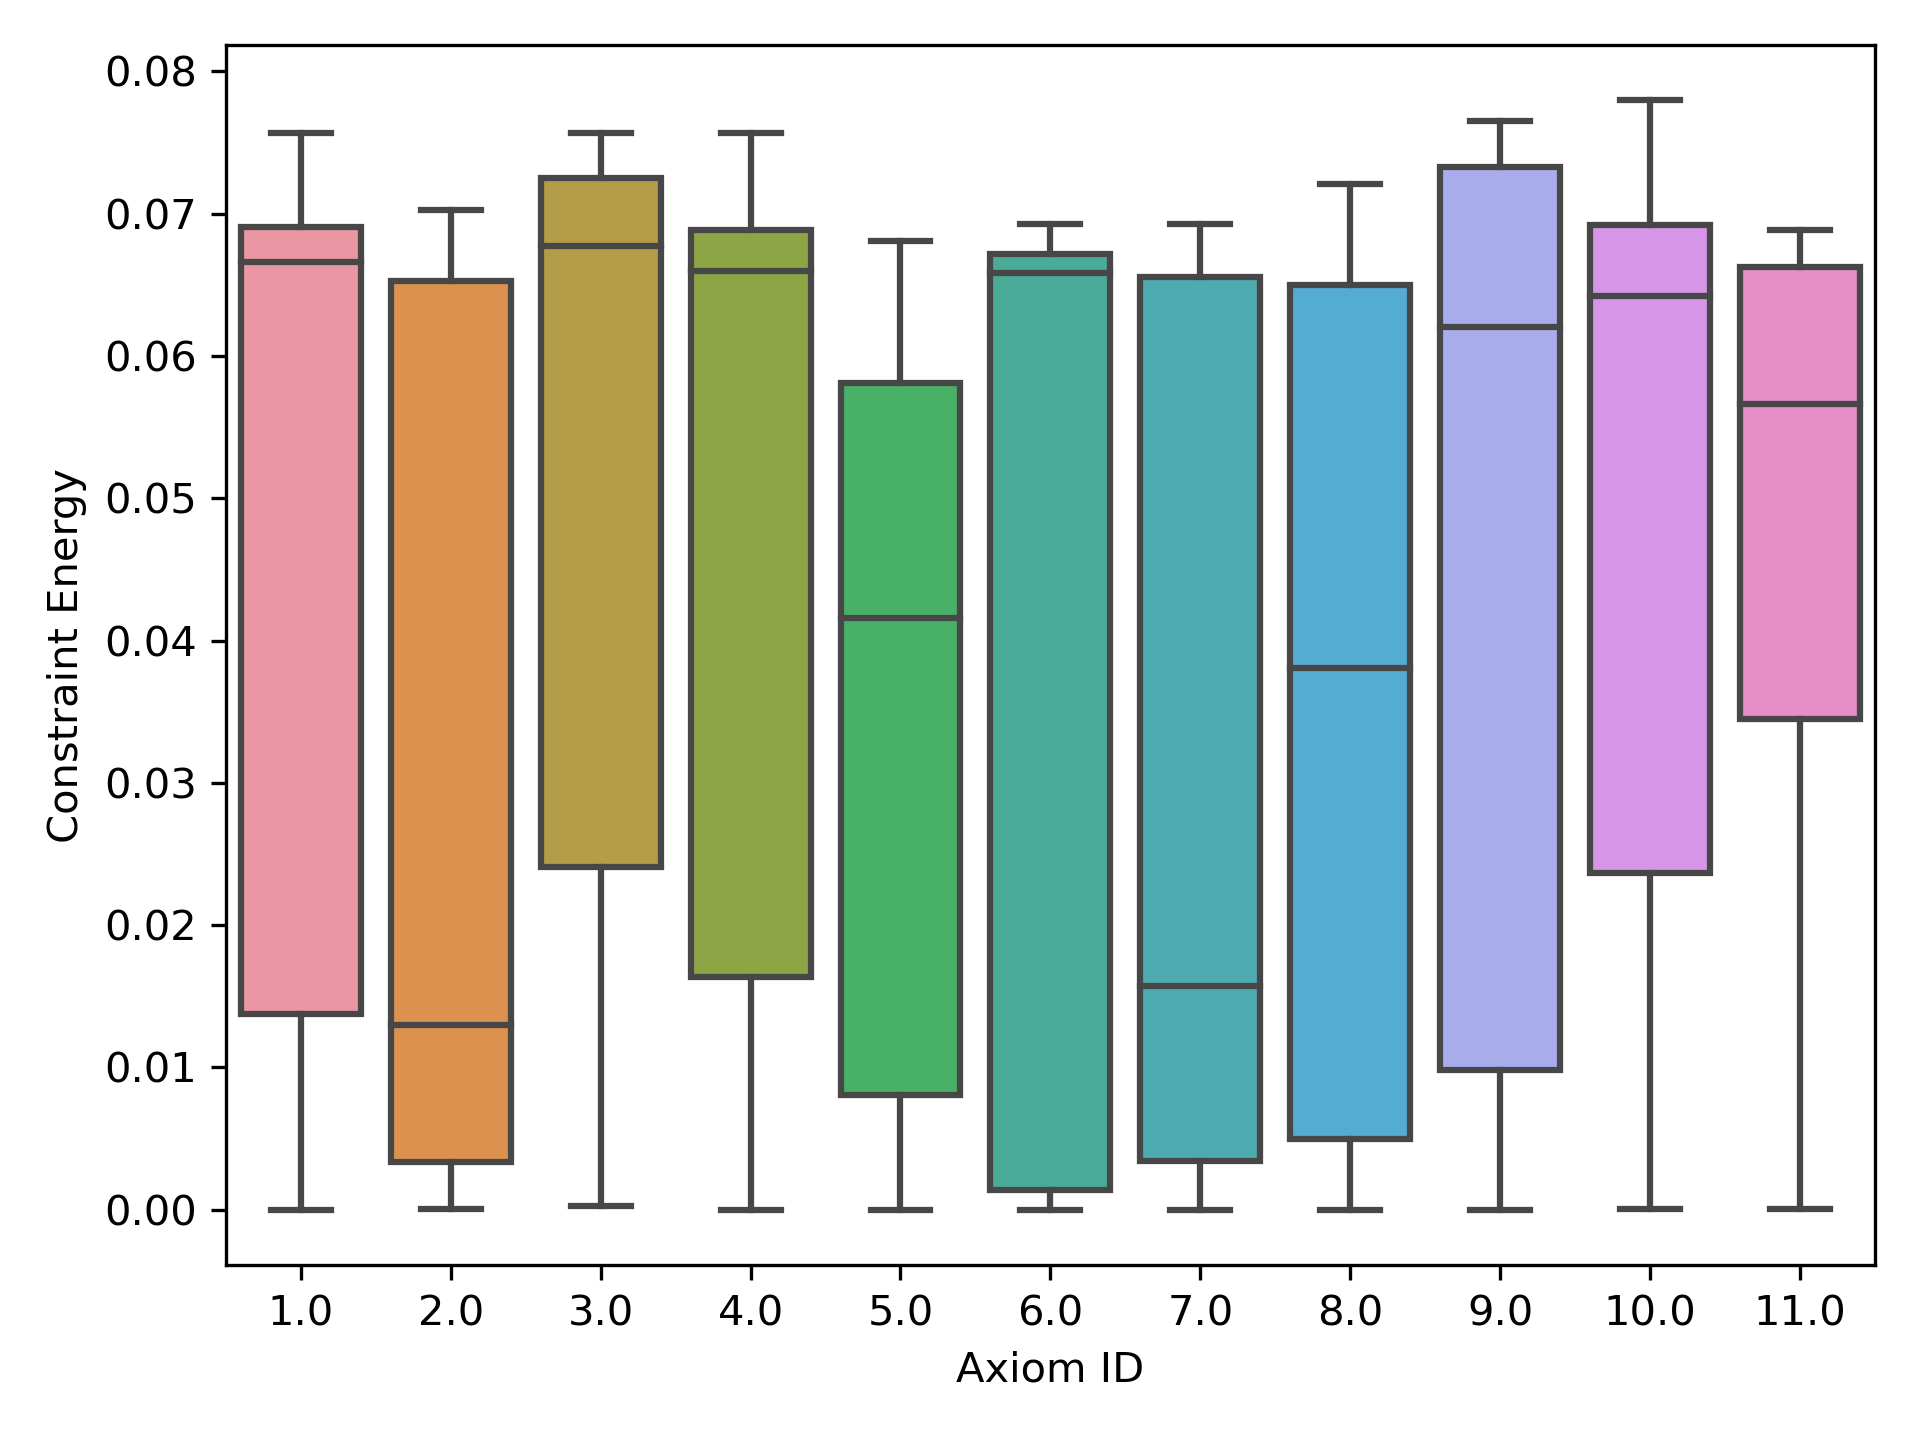
\includegraphics[width=\textwidth]{aid_vs_ce.png}
		\caption{Axiom ID vs constraint energy}
	\end{subfigure}
	\hfill
	\begin{subfigure}[t]{0.45\textwidth}
		\centering
		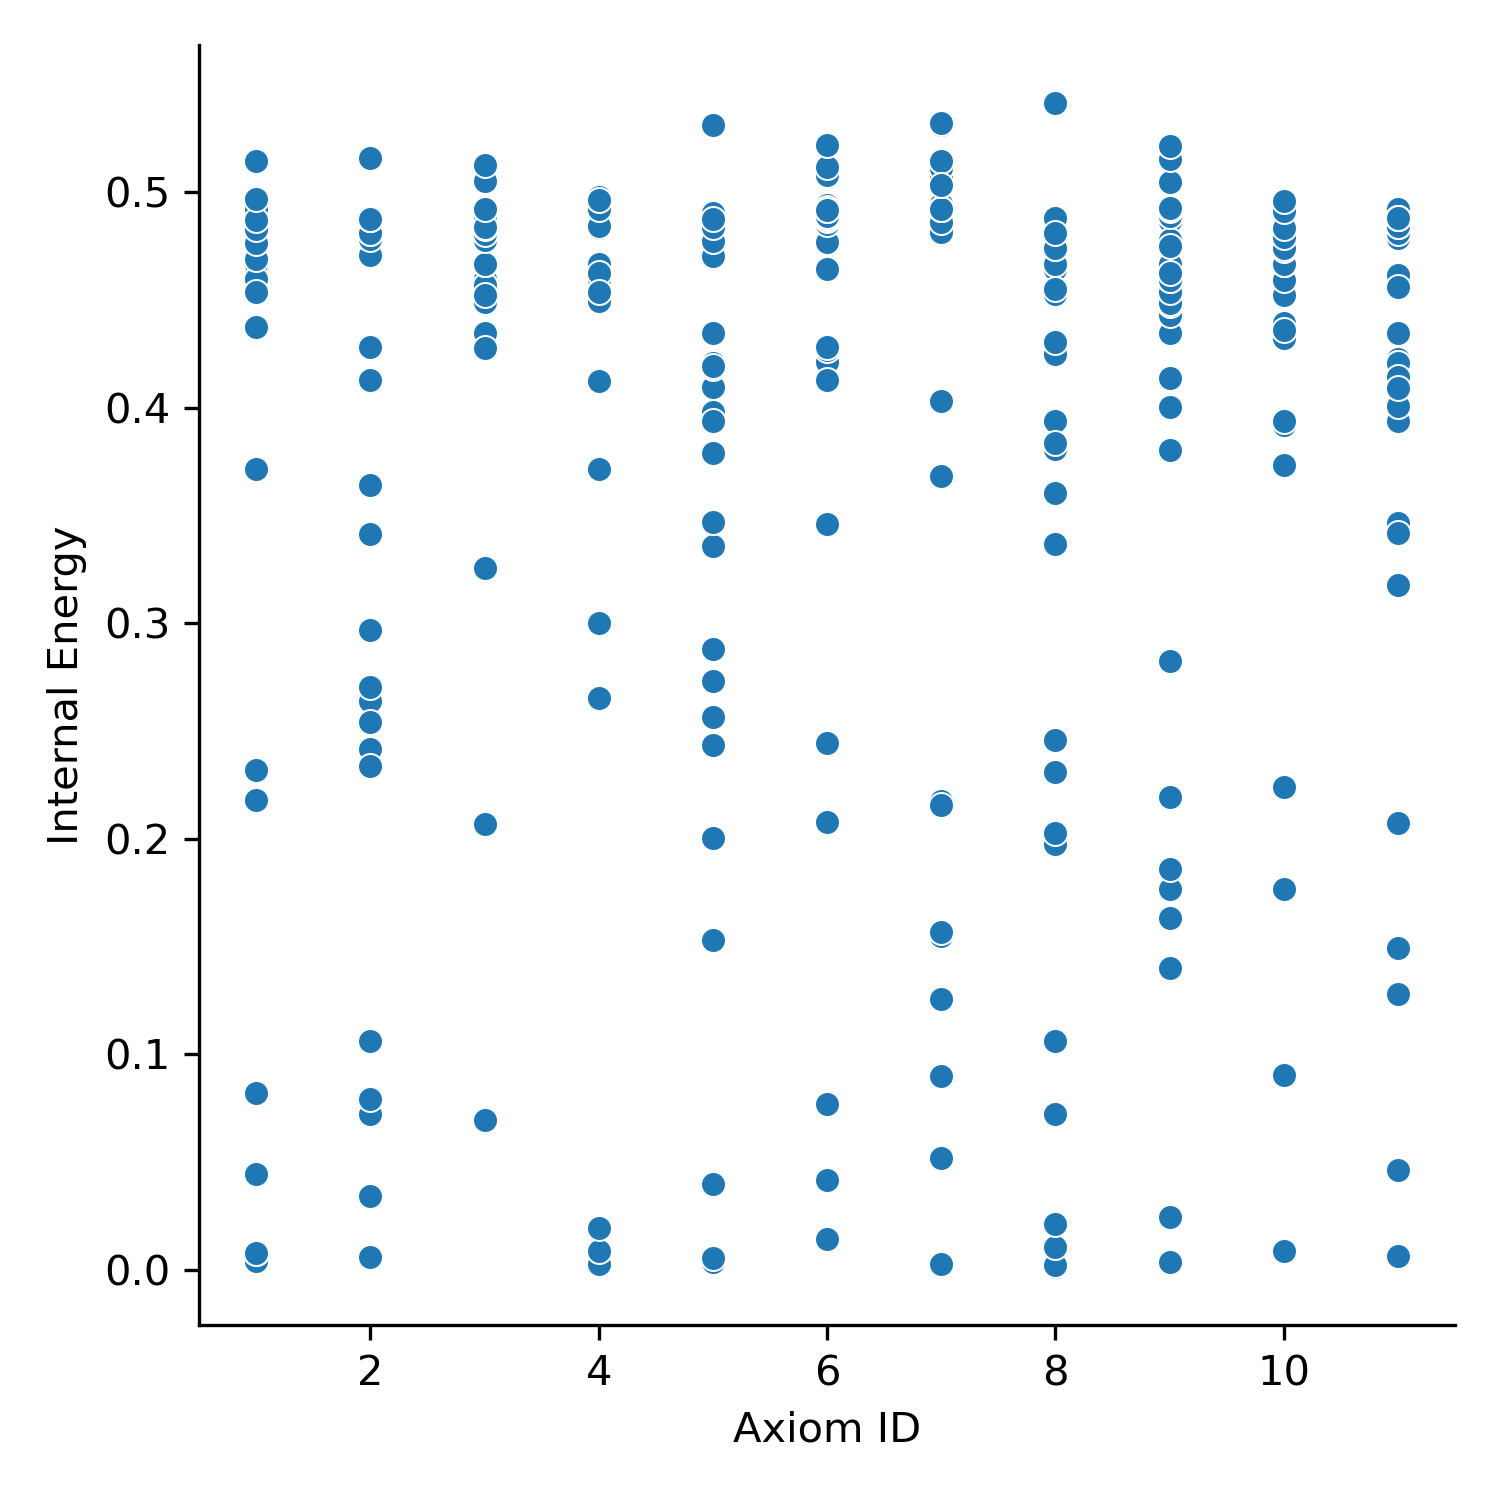
\includegraphics[width=\textwidth]{aid_vs_ie.png}
		\caption{Axiom ID vs internal energy}
	\end{subfigure}
	\hfill
	\begin{subfigure}[t]{0.45\textwidth}
		\centering
		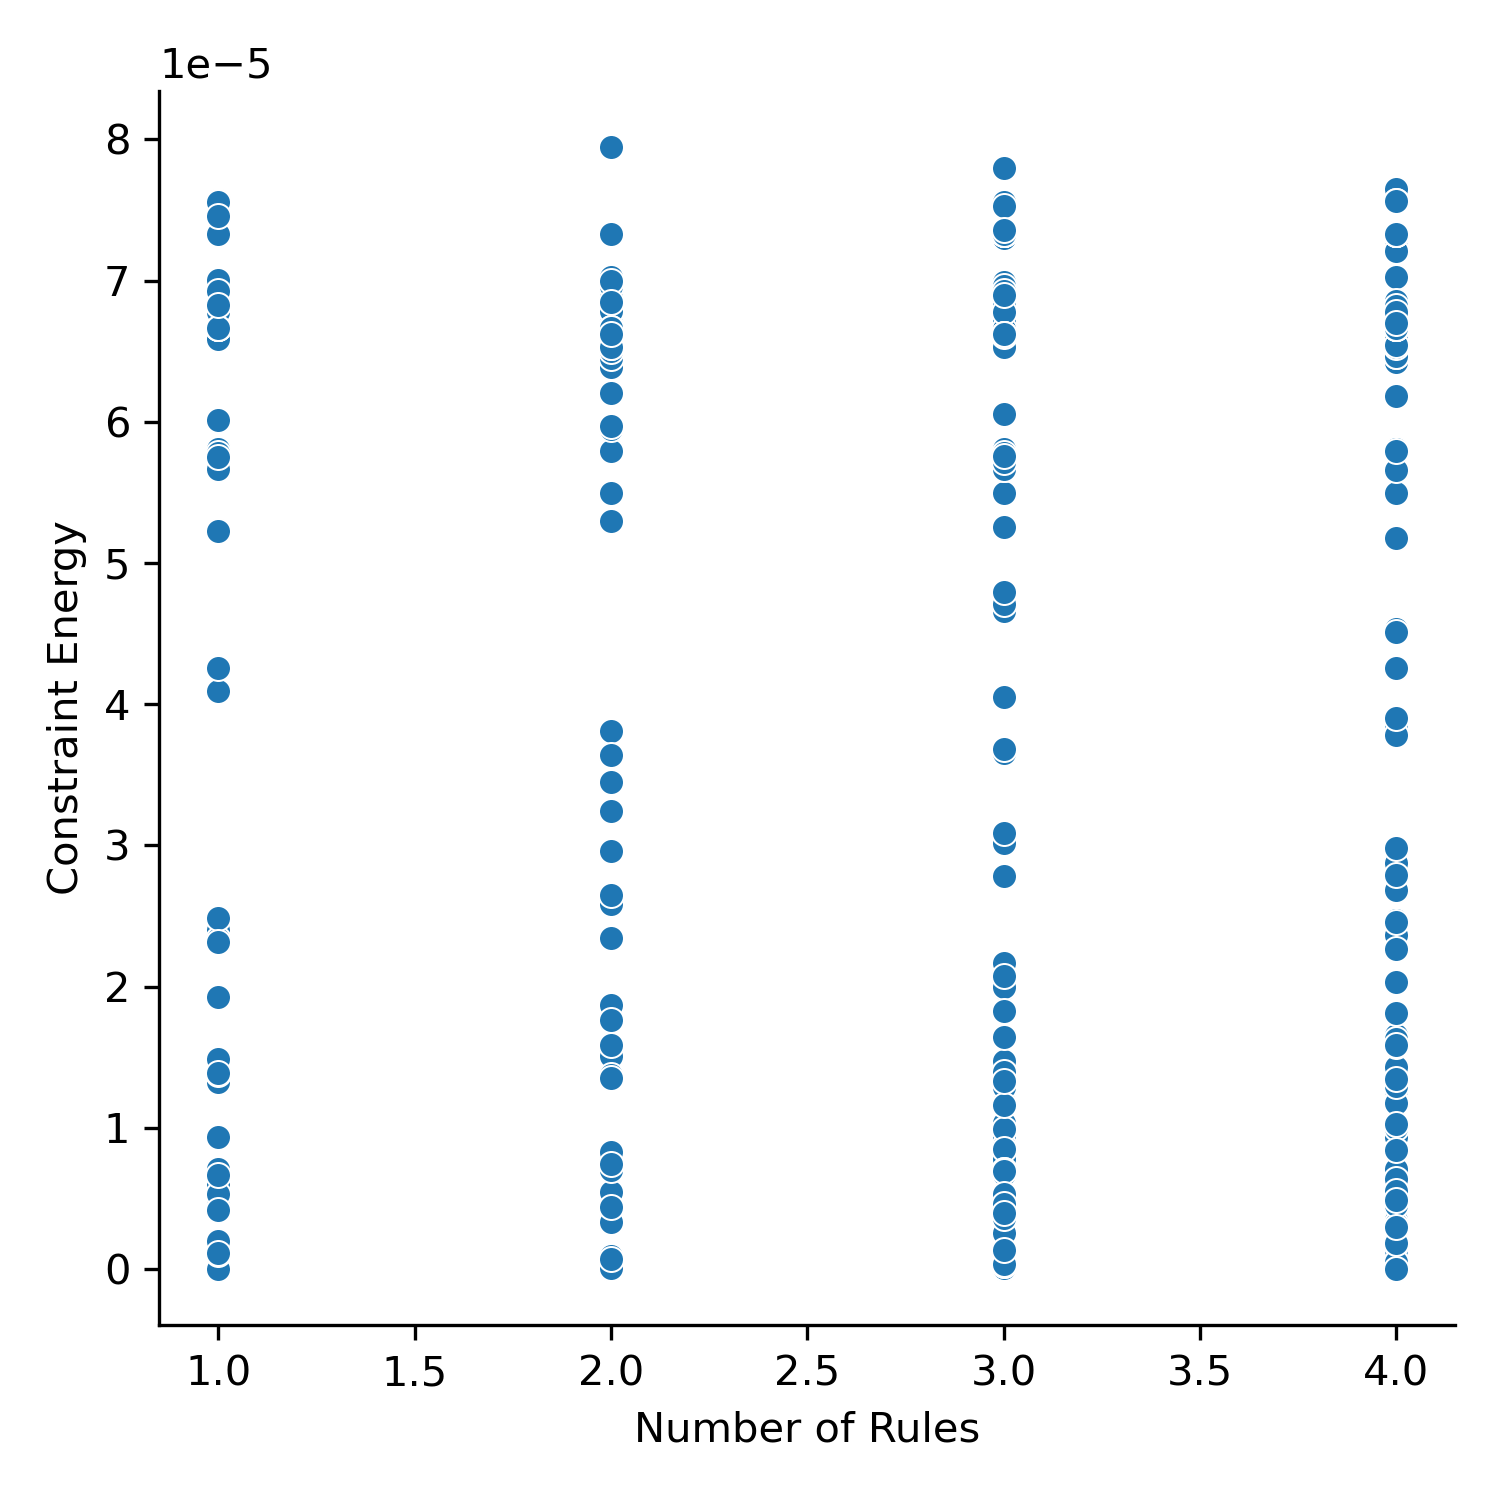
\includegraphics[width=\textwidth]{nor_vs_ce.png}
		\caption{Number of rules vs constraint energy}
	\end{subfigure}
	\hfill
	\begin{subfigure}[t]{0.45\textwidth}
		\centering
		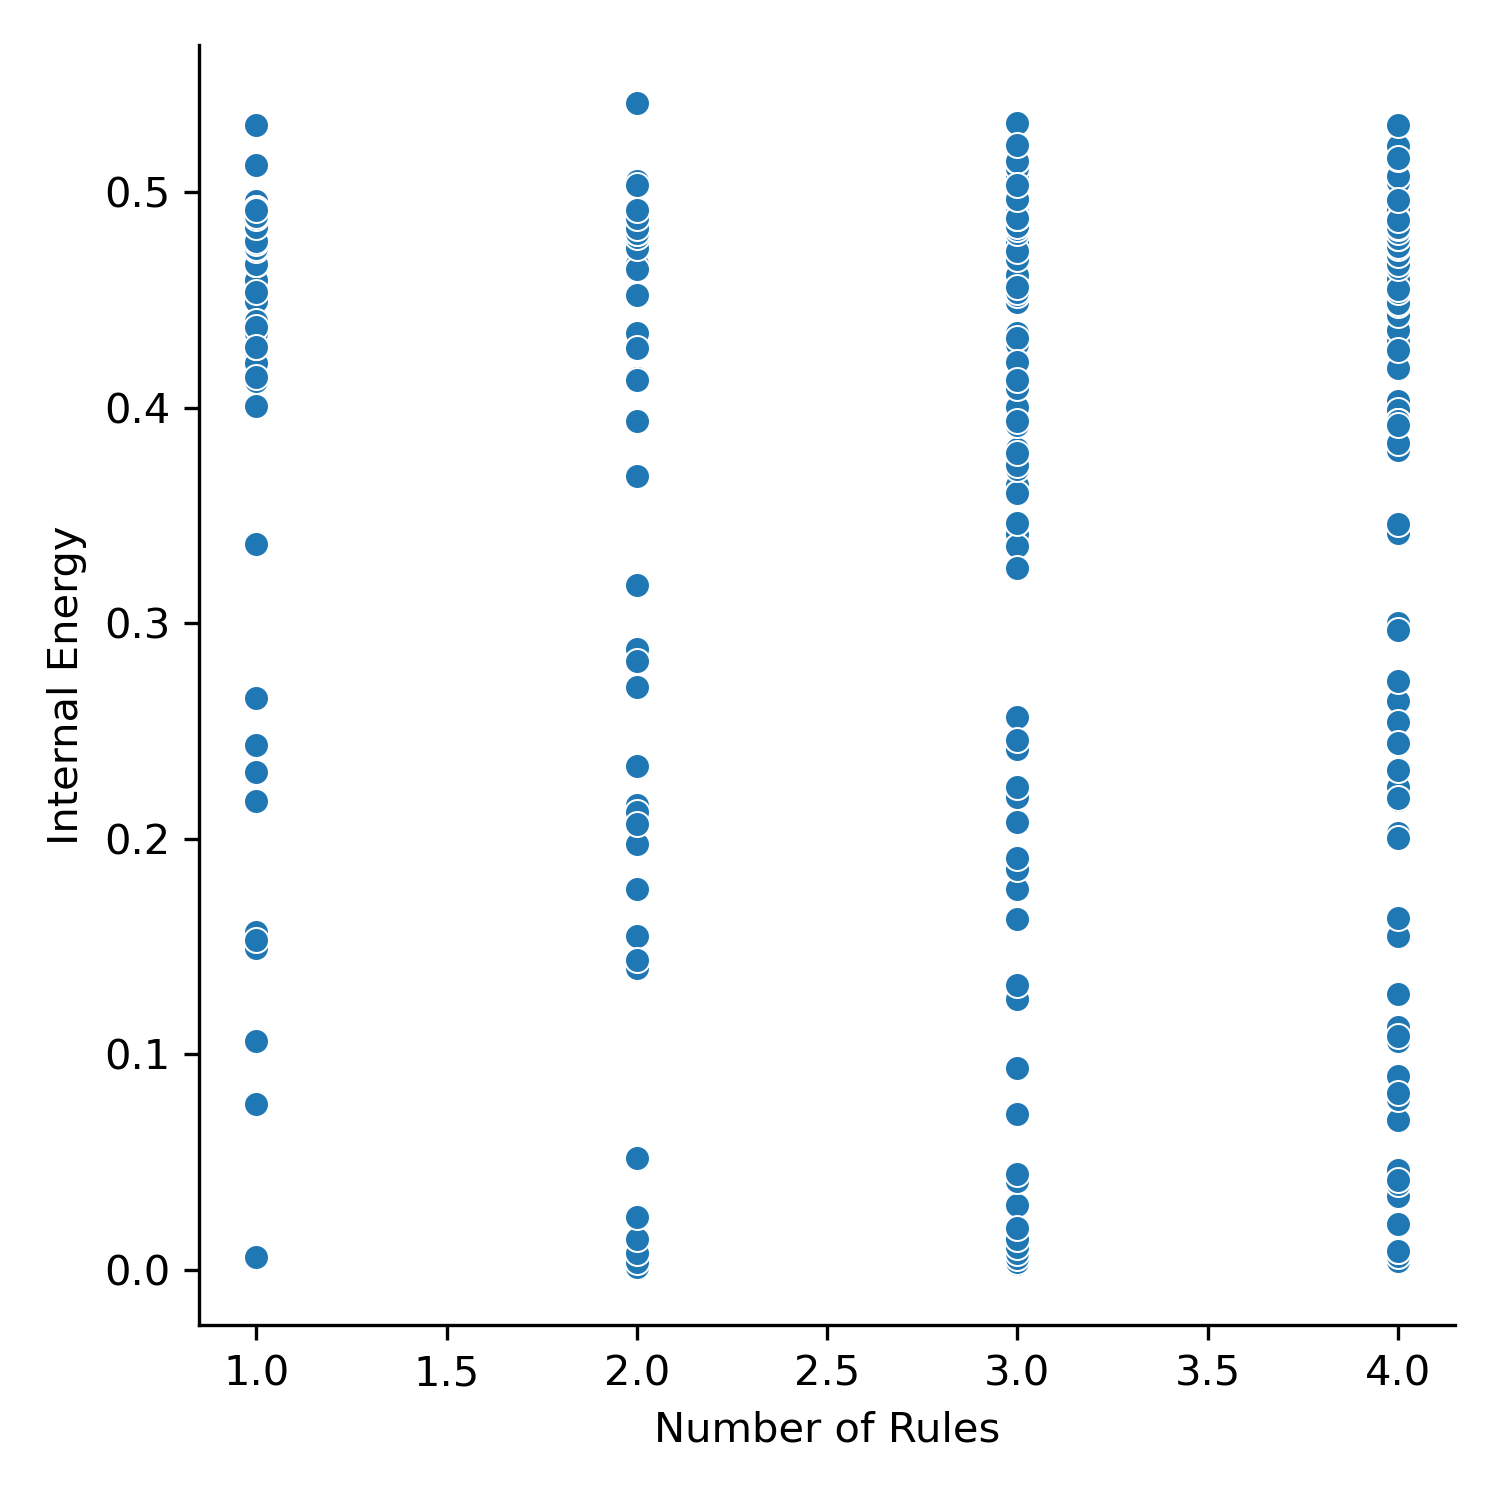
\includegraphics[width=\textwidth]{nor_vs_ie.png}
		\caption{Number of rules vs internal energy}
	\end{subfigure}
	\hfill
	\begin{subfigure}[t]{0.45\textwidth}
		\centering
		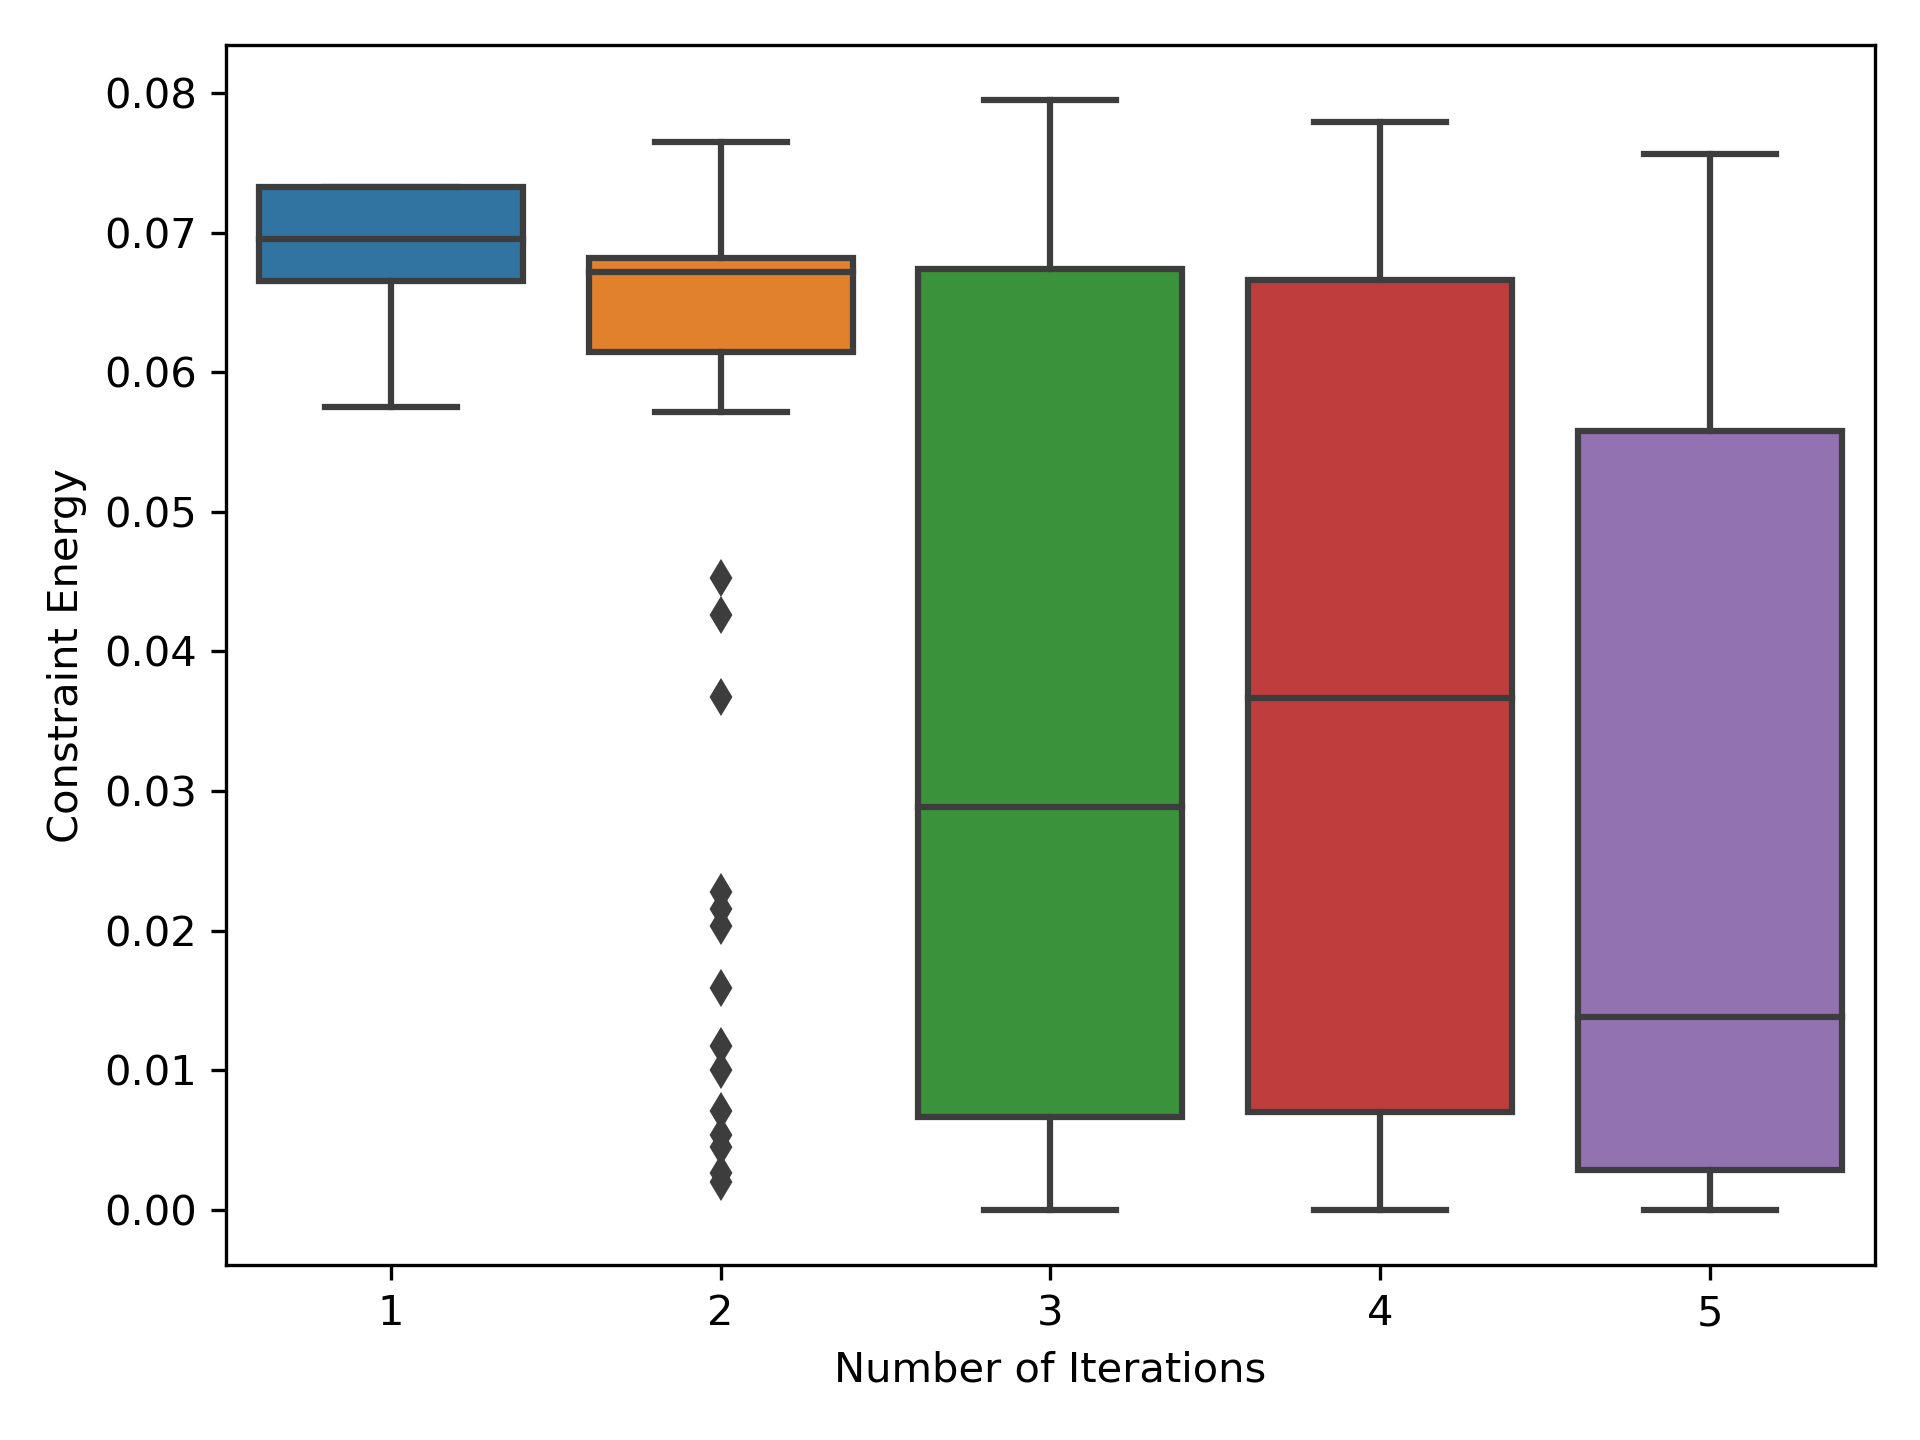
\includegraphics[width=\textwidth]{noi_vs_ce.png}
		\caption{Number of iterations vs constraint energy}
	\end{subfigure}
	\hfill
	\begin{subfigure}[t]{0.45\textwidth}
		\centering
		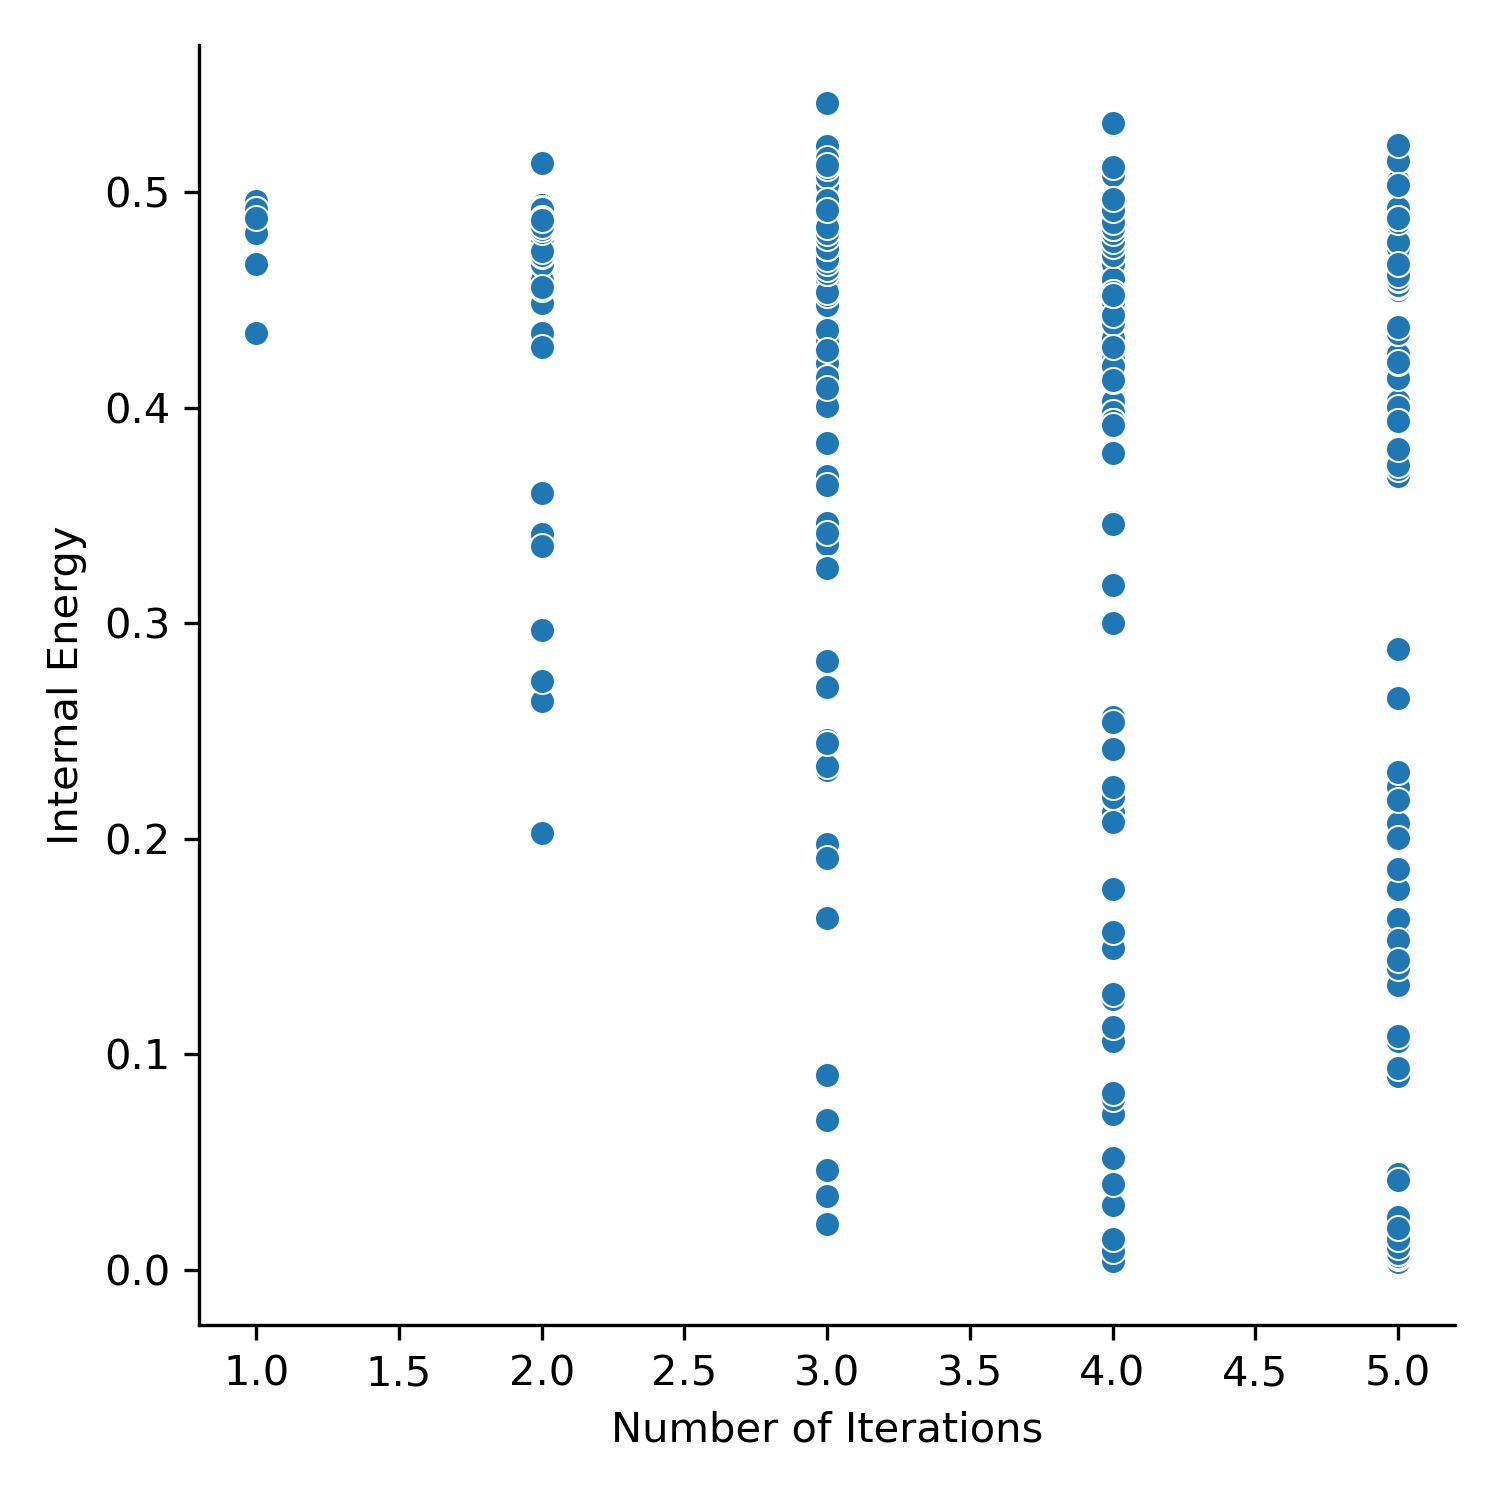
\includegraphics[width=\textwidth]{noi_vs_ie.png}
		\caption{Number of iterations vs internal energy}
	\end{subfigure}
	\caption[L-System parameters vs system energies]{L-System parameters vs constraint and internal energy (\si{mJ}) box-and-whisker plots}
	\label{fig:ls_v_e}
\end{figure}

\begin{figure}[H]
	\centering
	\begin{subfigure}[c]{0.45\textwidth}
		\centering
		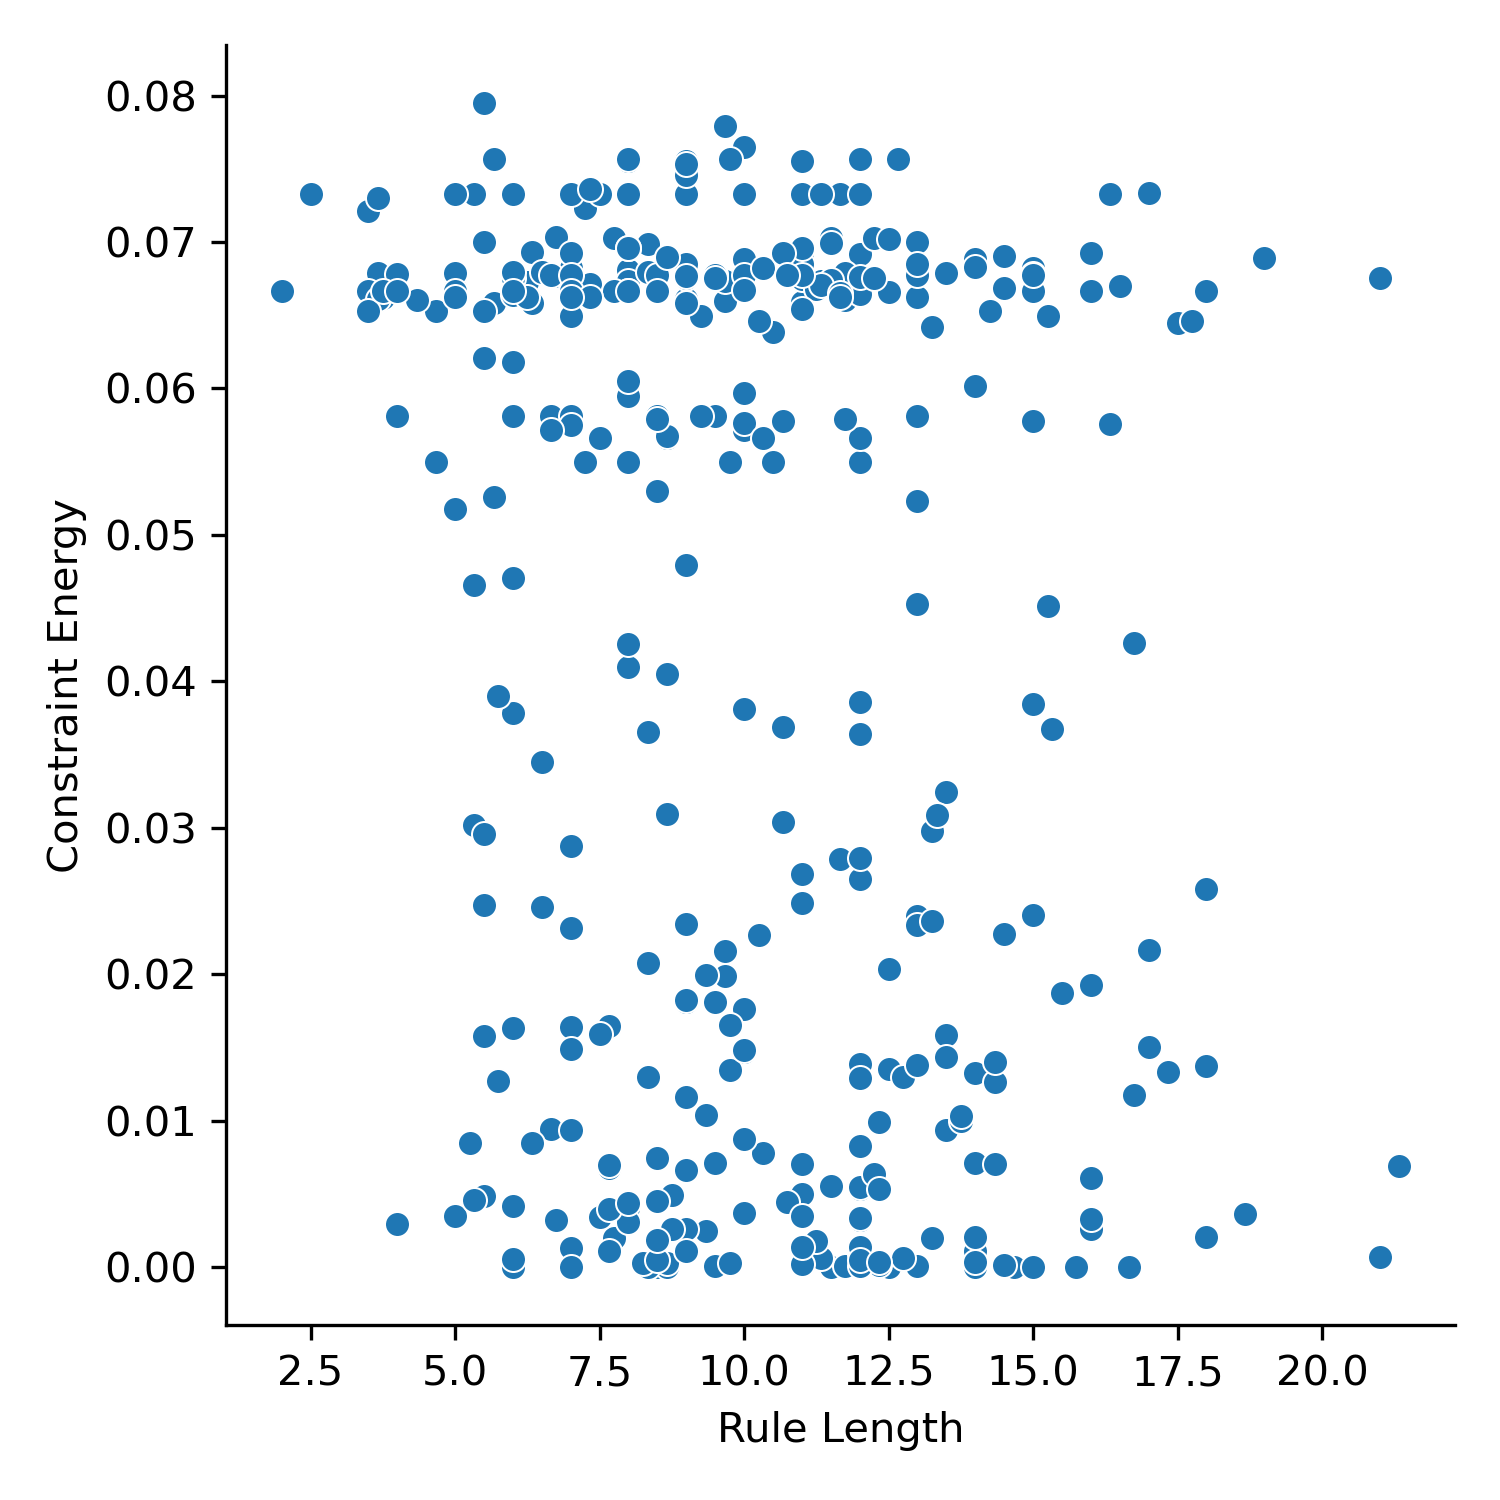
\includegraphics[width=\textwidth]{rl_vs_ce.png}
		\caption{Rule length vs constraint energy}
	\end{subfigure}
	\hfill
	\begin{subfigure}[c]{0.45\textwidth}
		\centering
		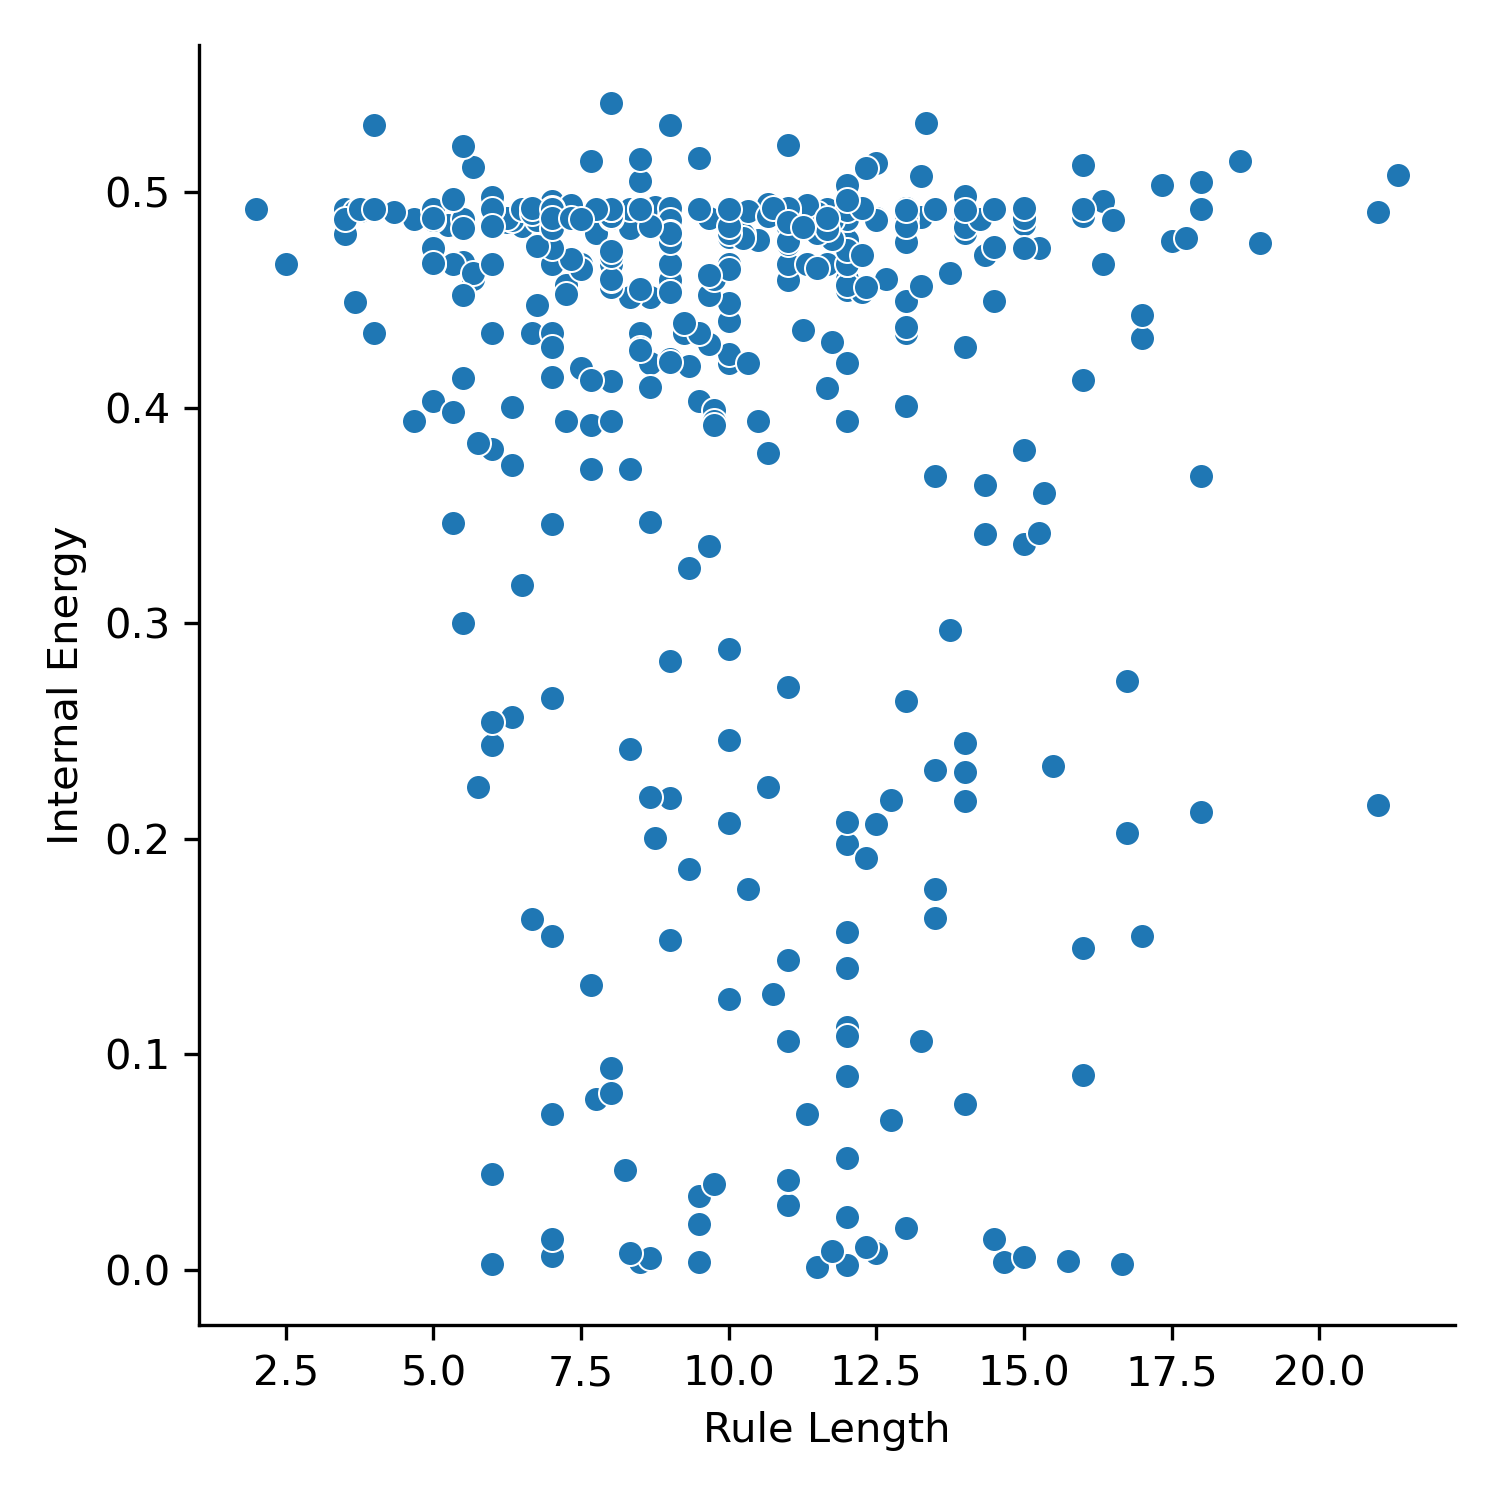
\includegraphics[width=\textwidth]{rl_vs_ie.png}
		\caption{Rule length vs internal energy}
	\end{subfigure}
	\caption[Rule length vs system energies]{Average rule length vs constraint and internal energy (\si{mJ}) scatter plots}
	\label{fig:rl_v_e}
\end{figure}

\subsection{CPPN Unit Generation}

Parameter ranges are outlined in Table~\ref{tab:cppnmc}.

% Please add the following required packages to your document preamble:
% \usepackage{booktabs}
\begin{table}[H]
\centering
\caption{CPPN unit generation parameters for a Monte Carlo analysis}
\label{tab:cppnmc}
\begin{tabular}{@{}lcc@{}}
\toprule
\multicolumn{1}{c}{\textbf{Parameter}} & \textbf{Minimum} & \textbf{Maximum} \\ \midrule
Seed                                   & 1                & 1000             \\
Model ID                               & 1                & N/A              \\
Scale                                  & 1                & N/A              \\
Number of hidden layers                & 2                & 10               \\
Size of the initial hidden layer       & 2                & 32               \\
Element removal threshold              & 0                & 100              \\ \bottomrule
\end{tabular}
\end{table}

Figure~\ref{fig:nhl_v_e} contains box-and-whisker plots relating the number of hidden layers to the system energies. The number of hidden layers has no discernible relationship with the system energies. Figure~\ref{fig:sihl_v_e} contains scatter plots relating the size of the initial hidden layer to the system energies. There is no strong relationship between the size of the initial hidden layer and the system energies.

\begin{figure}[H]
	\centering
	\begin{subfigure}[t]{0.45\textwidth}
		\centering
		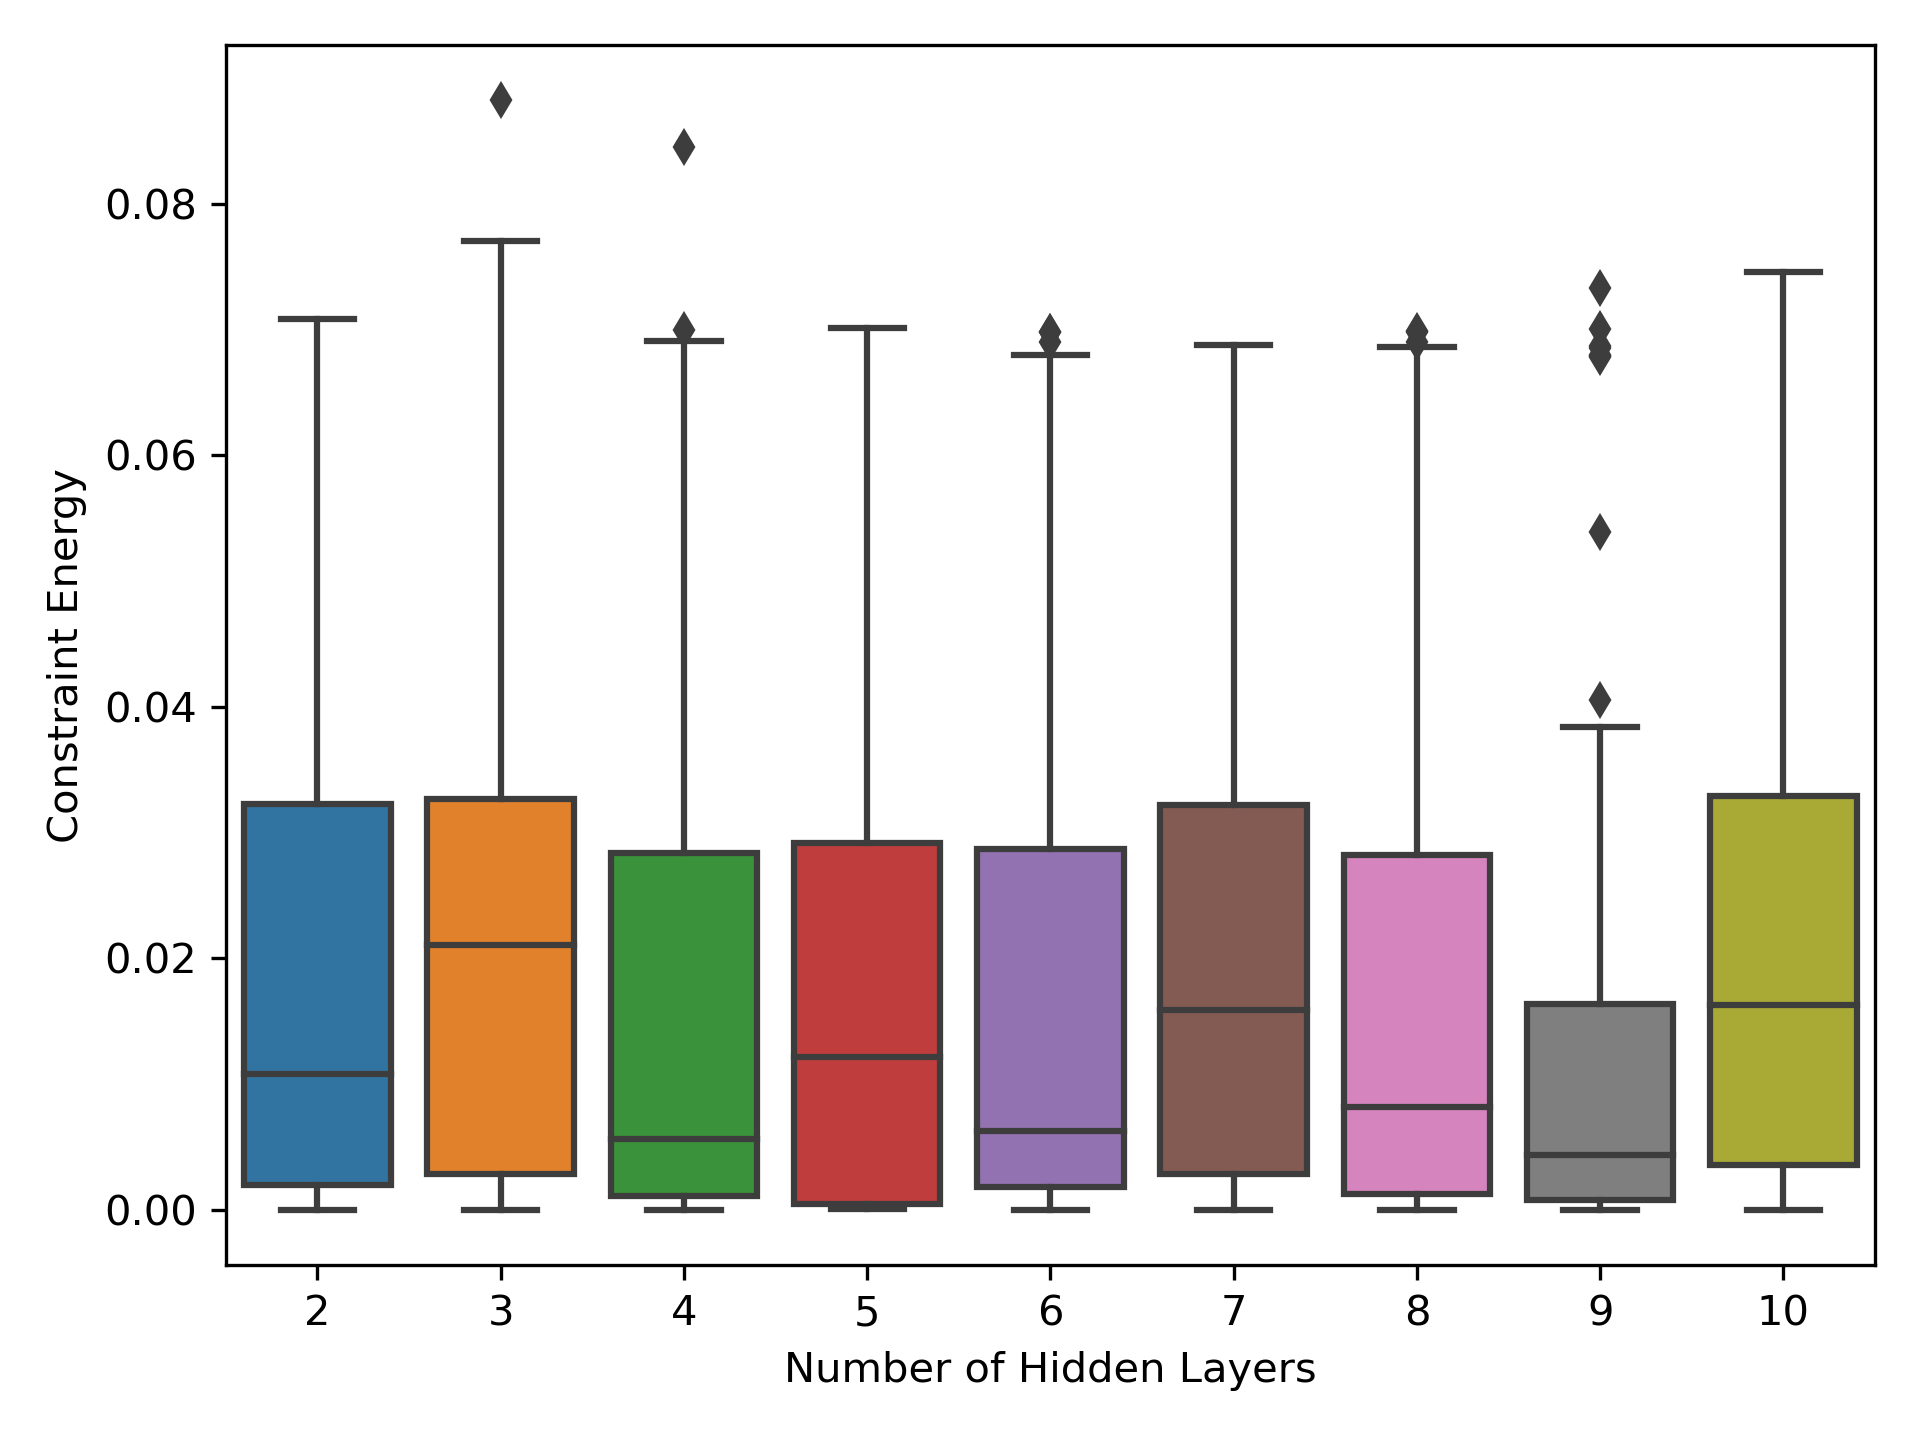
\includegraphics[width=\textwidth]{nhl_vs_ce.png}
		\caption{Number of hidden layers vs constraint energy}
	\end{subfigure}
	\hfill
	\begin{subfigure}[t]{0.45\textwidth}
		\centering
		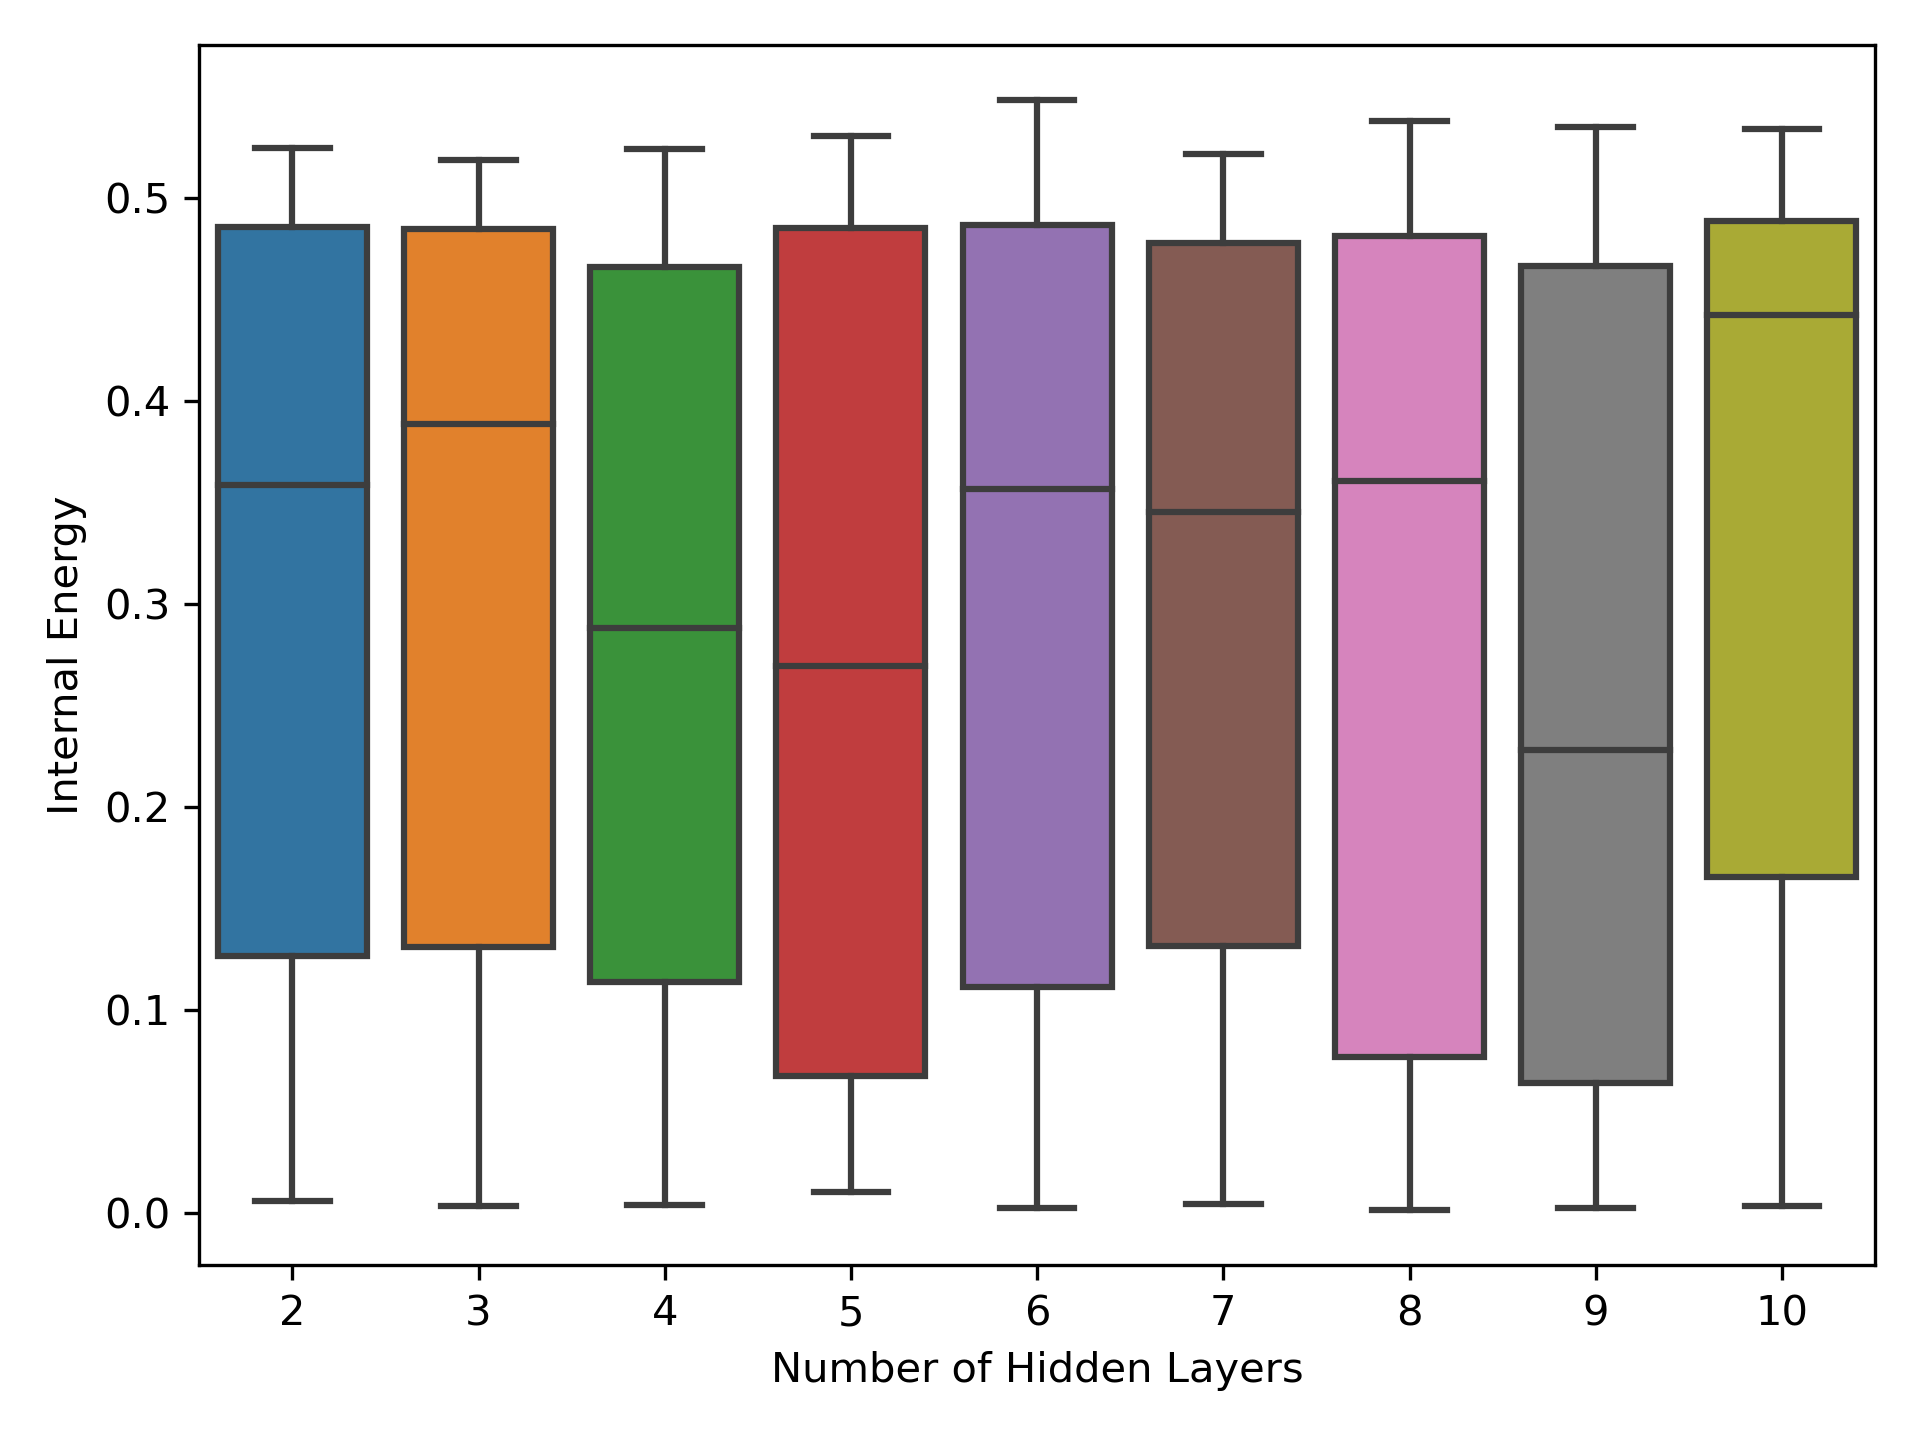
\includegraphics[width=\textwidth]{nhl_vs_ie.png}
		\caption{Number of hidden layers vs internal energy}
	\end{subfigure}
	\caption[Number of hidden layers vs system energies]{Number of hidden layers vs constraint and internal energy (\si{mJ}) box-and-whisker plots}
	\label{fig:nhl_v_e}
\end{figure}

\begin{figure}[H]
	\centering
	\begin{subfigure}[t]{0.45\textwidth}
		\centering
		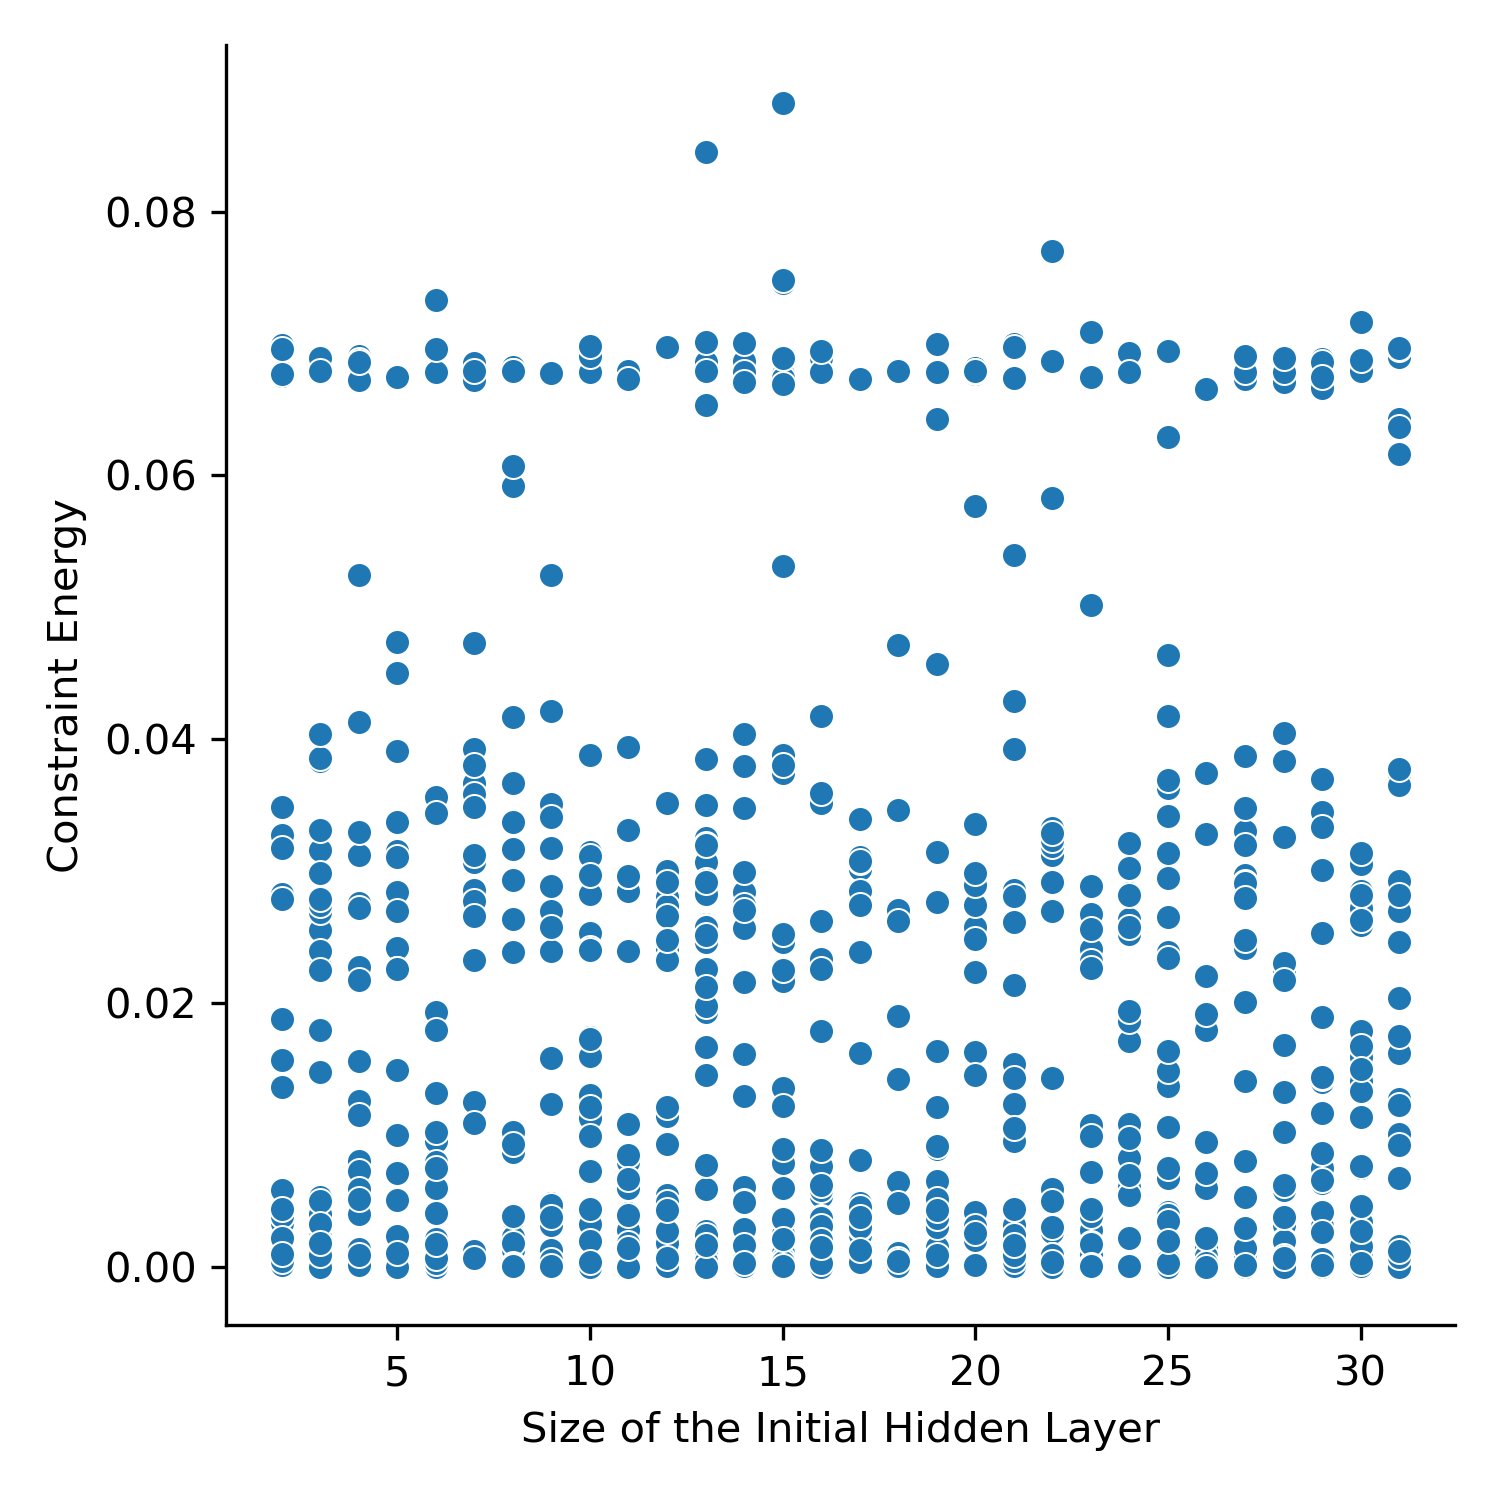
\includegraphics[width=\textwidth]{sihl_vs_ce.png}
		\caption{Size of the initial hidden layer vs constraint energy}
	\end{subfigure}
	\hfill
	\begin{subfigure}[t]{0.45\textwidth}
		\centering
		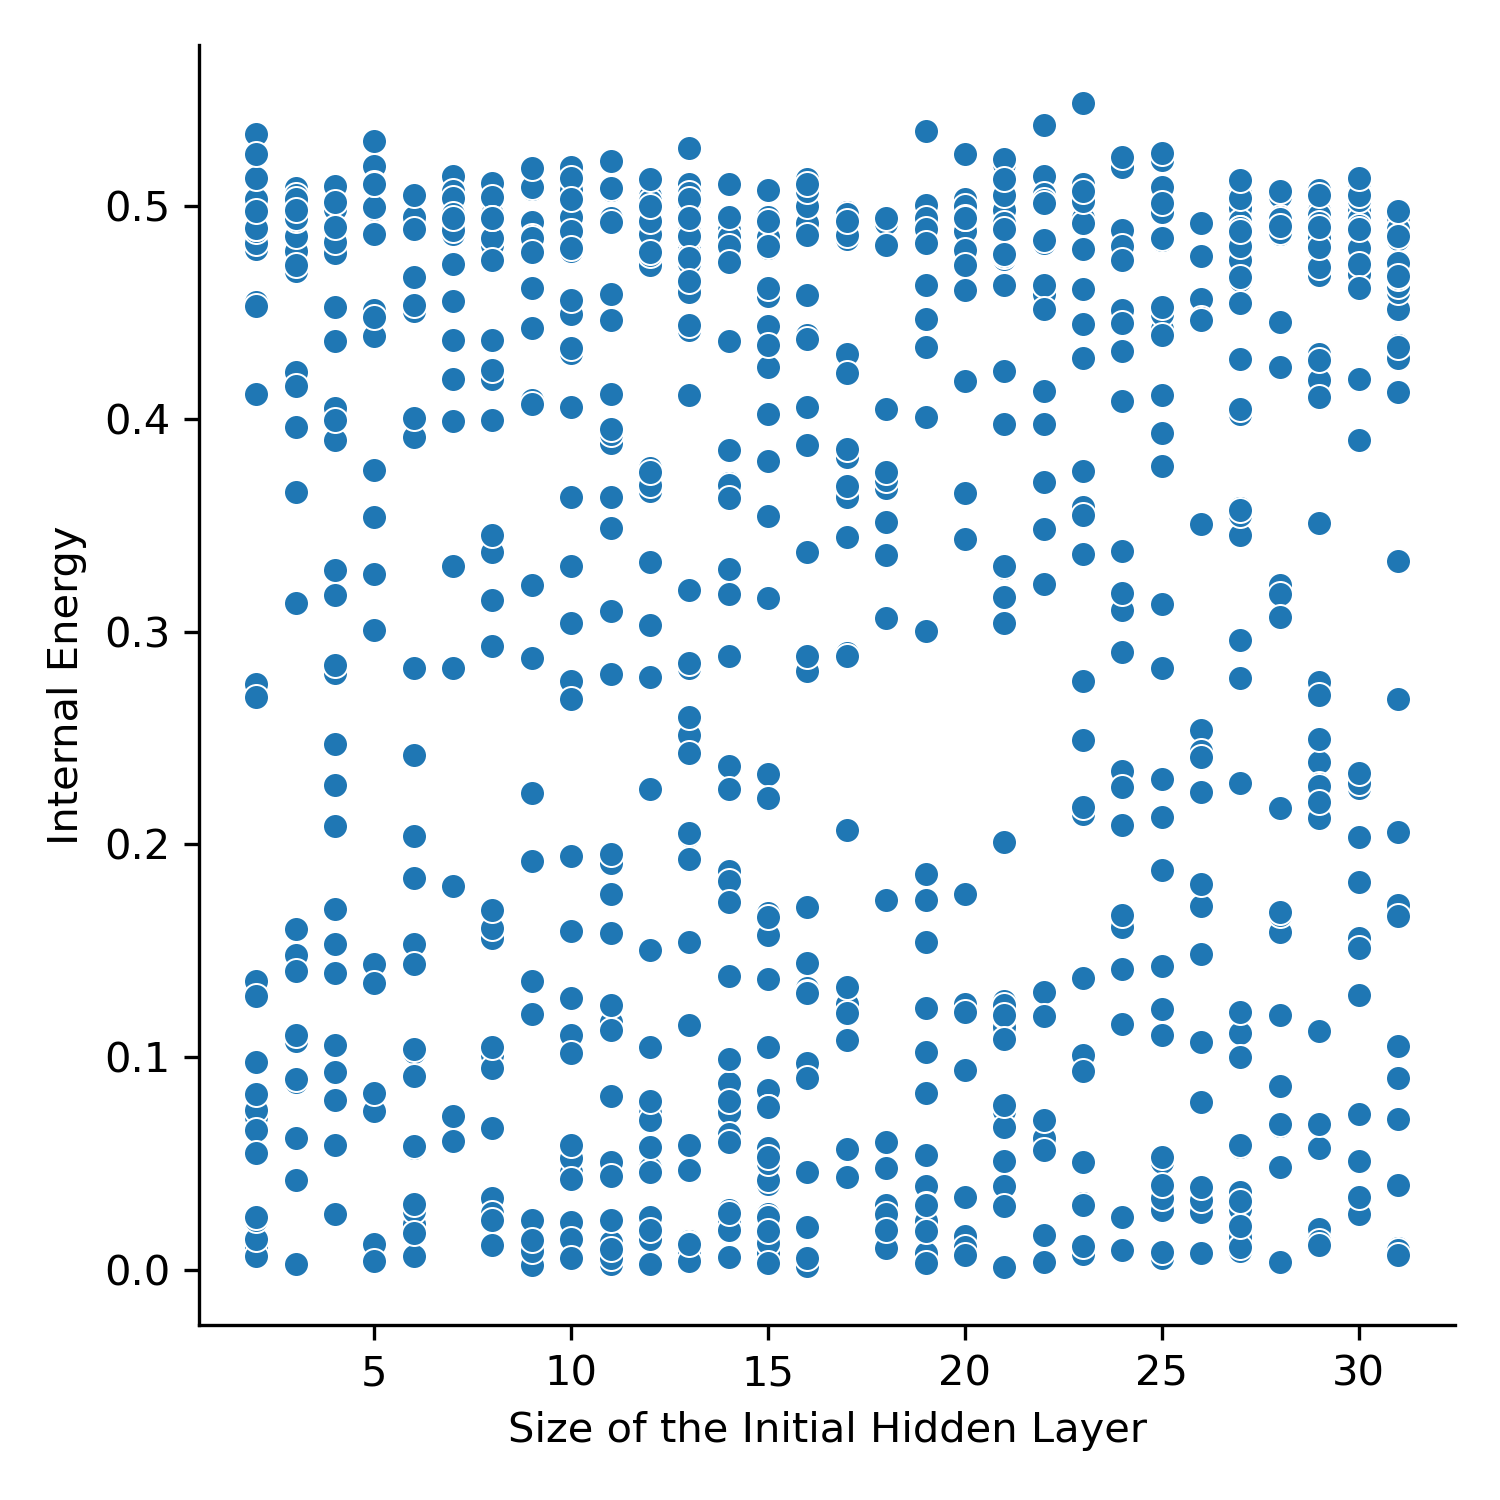
\includegraphics[width=\textwidth]{sihl_vs_ie.png}
		\caption{Size of the initial hidden layer vs internal energy}
	\end{subfigure}
	\caption[Size of the initial hidden layer vs system energies]{Size of the initial hidden layer vs constraint and internal energy (\si{mJ}) scatter plots}
	\label{fig:sihl_v_e}
\end{figure}

\subsection{Comparison}

The distribution of the constraint and internal energies for the three unit generation methods is compared in Figure~\ref{fig:ciecomp}.

\begin{figure}[H]
	\centering
	\begin{subfigure}[c]{0.45\textwidth}
		\centering
		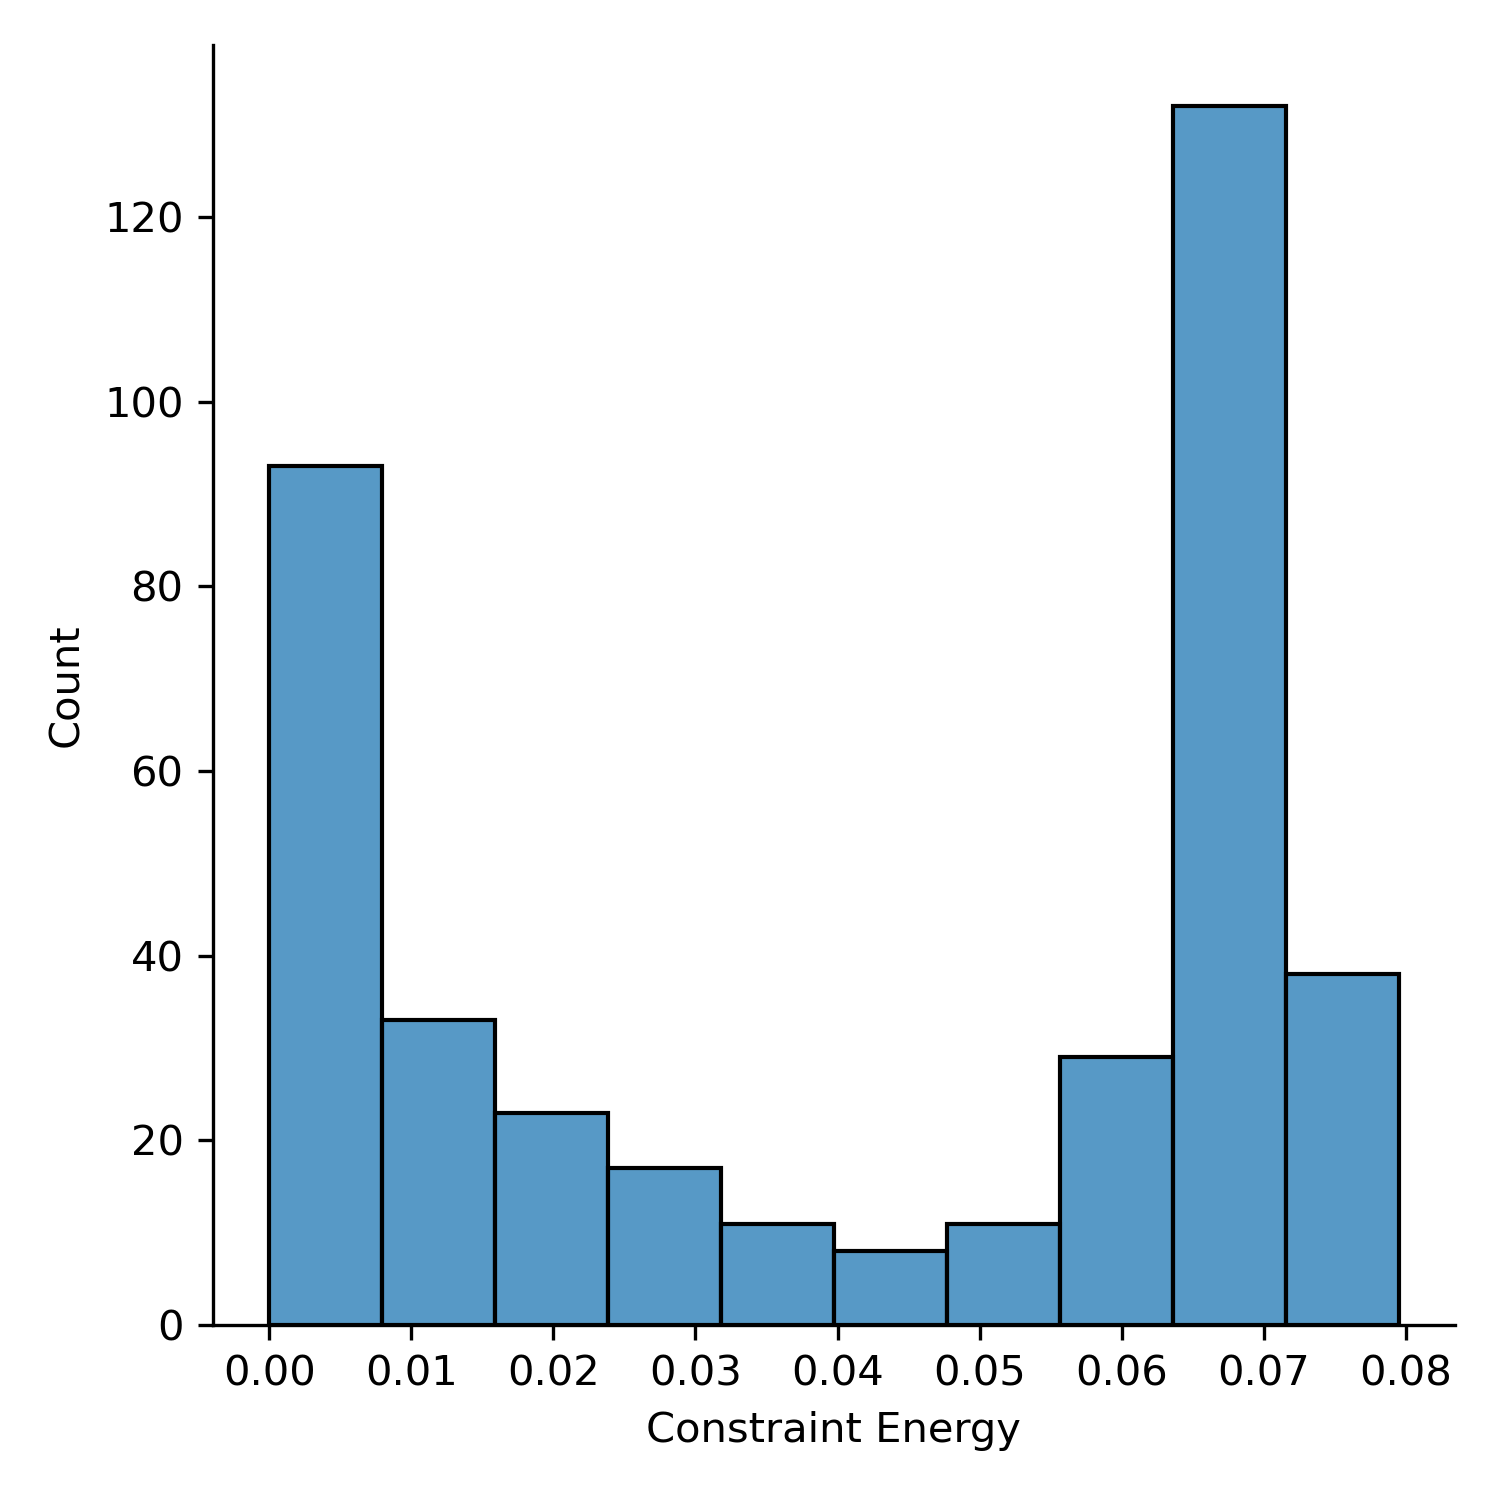
\includegraphics[width=\textwidth]{ce_ls.png}
		\caption{Constraint energy distribution of L-Systems}
	\end{subfigure}
	\hfill
	\begin{subfigure}[c]{0.45\textwidth}
		\centering
		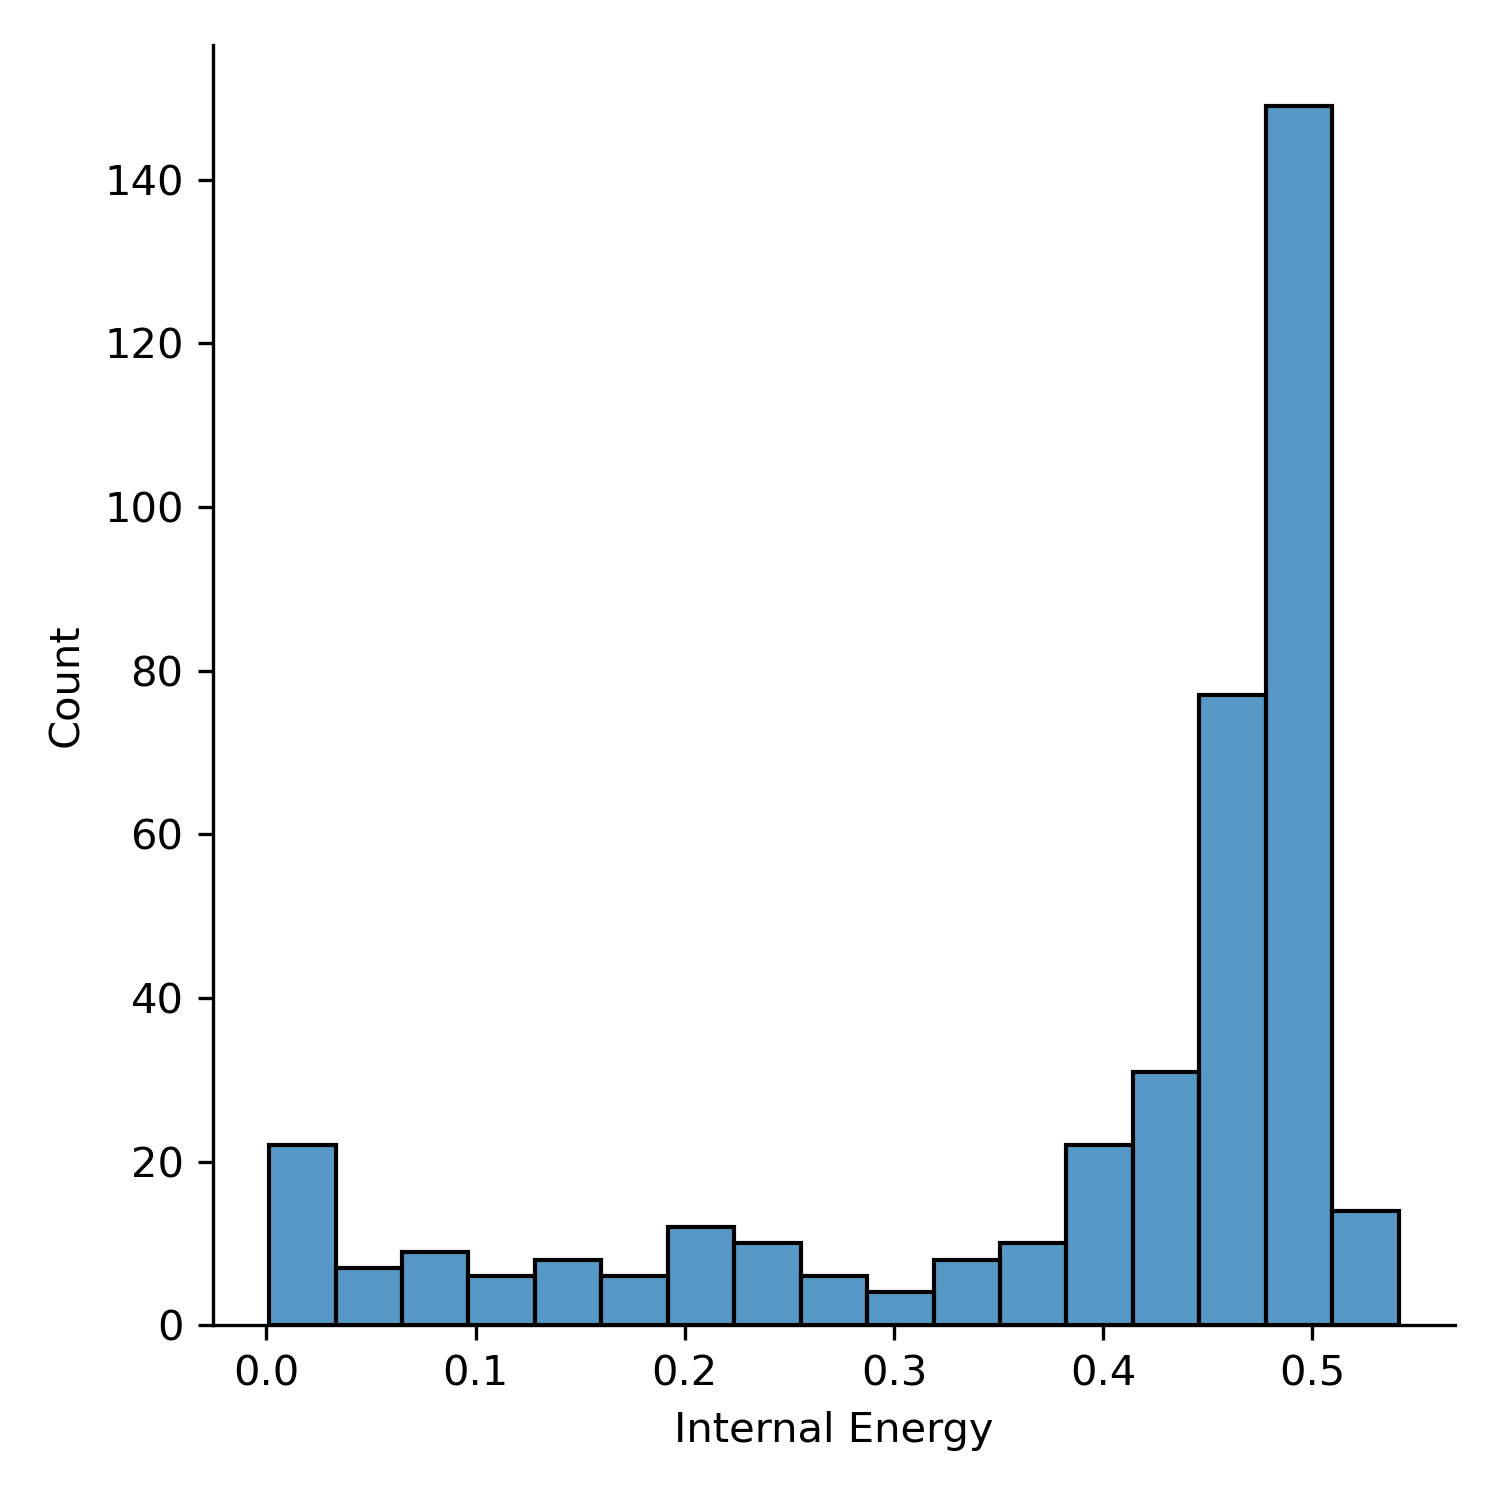
\includegraphics[width=\textwidth]{ie_ls.png}
		\caption{Internal energy distribution of L-Systems}
	\end{subfigure}
	\hfill
	\begin{subfigure}[c]{0.45\textwidth}
		\centering
		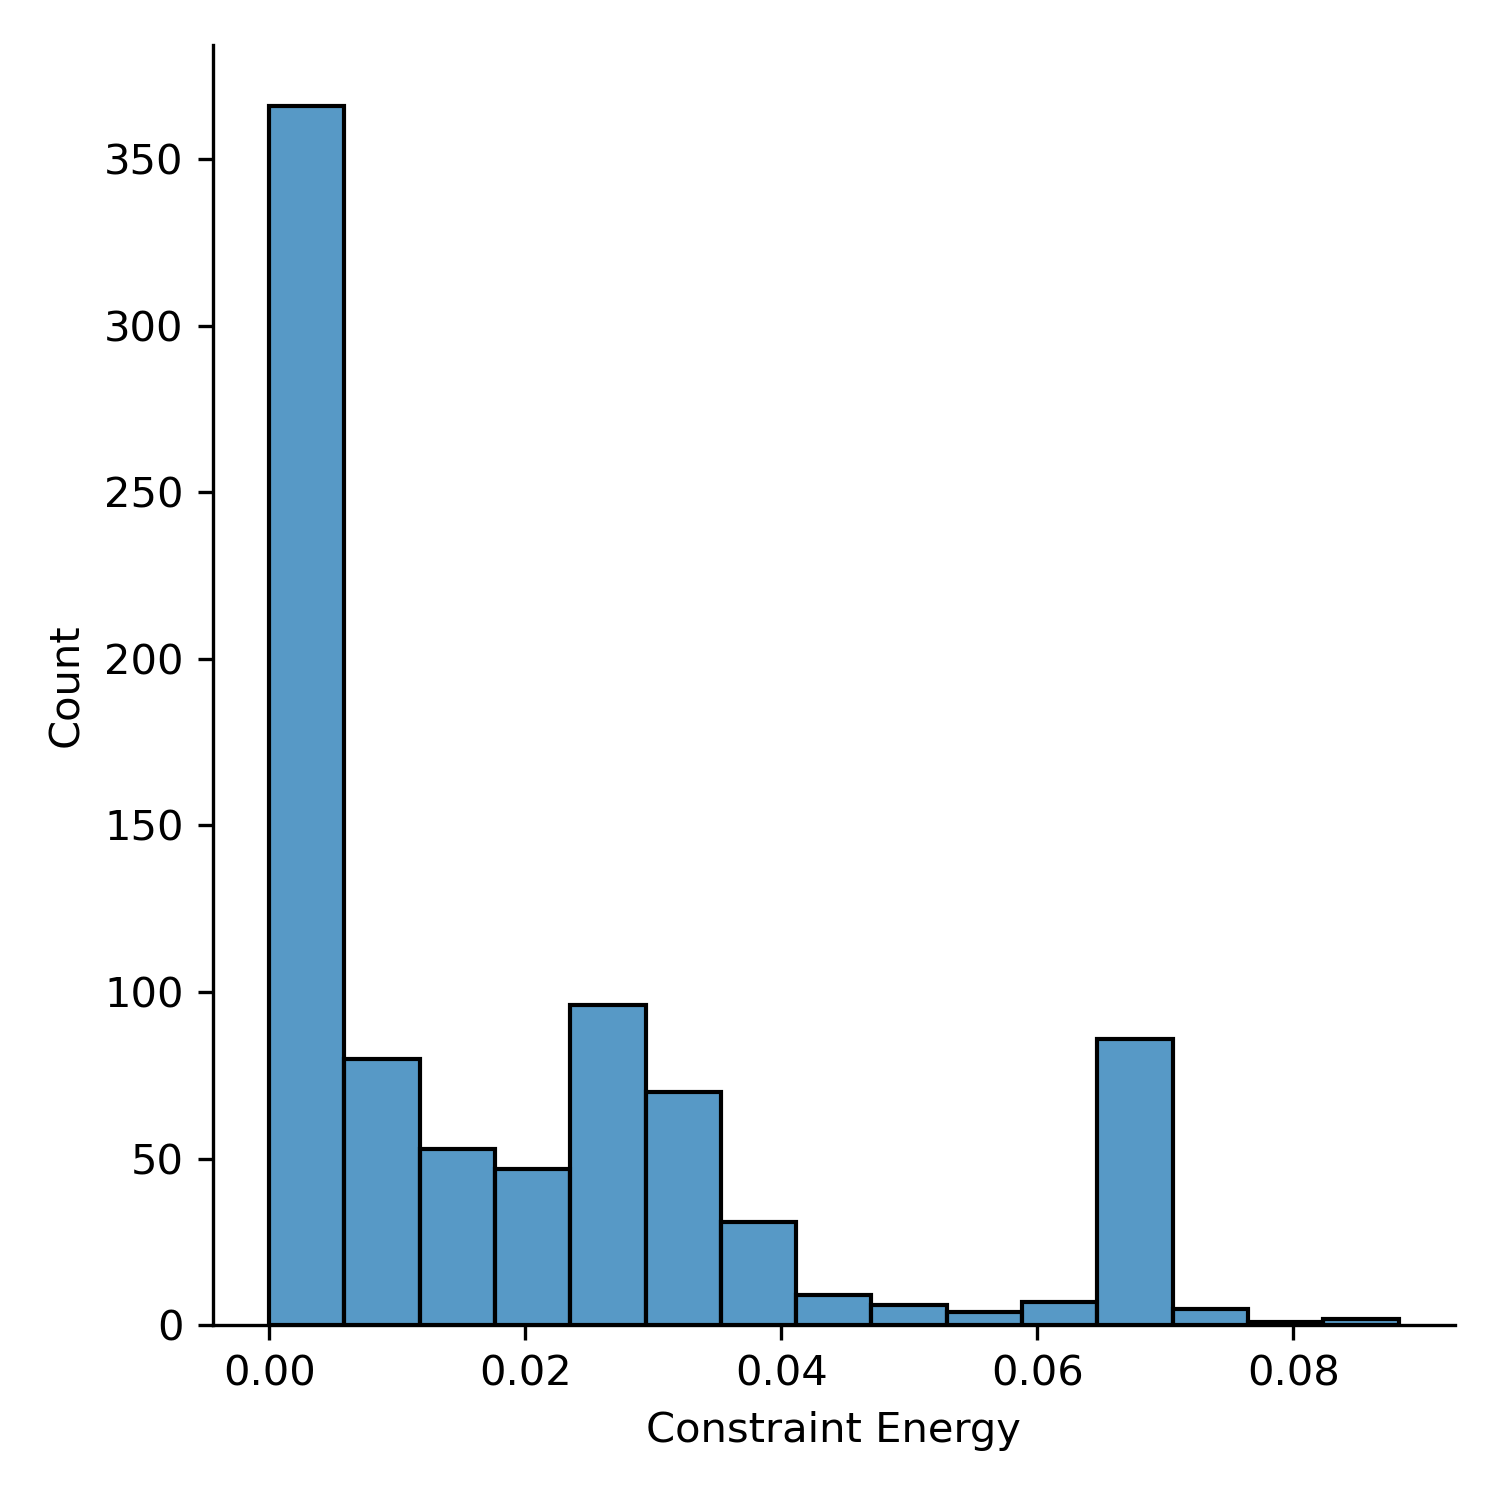
\includegraphics[width=\textwidth]{ce_cppn.png}
		\caption{Constraint energy distribution of CPPNs}
	\end{subfigure}
	\hfill
	\begin{subfigure}[c]{0.45\textwidth}
		\centering
		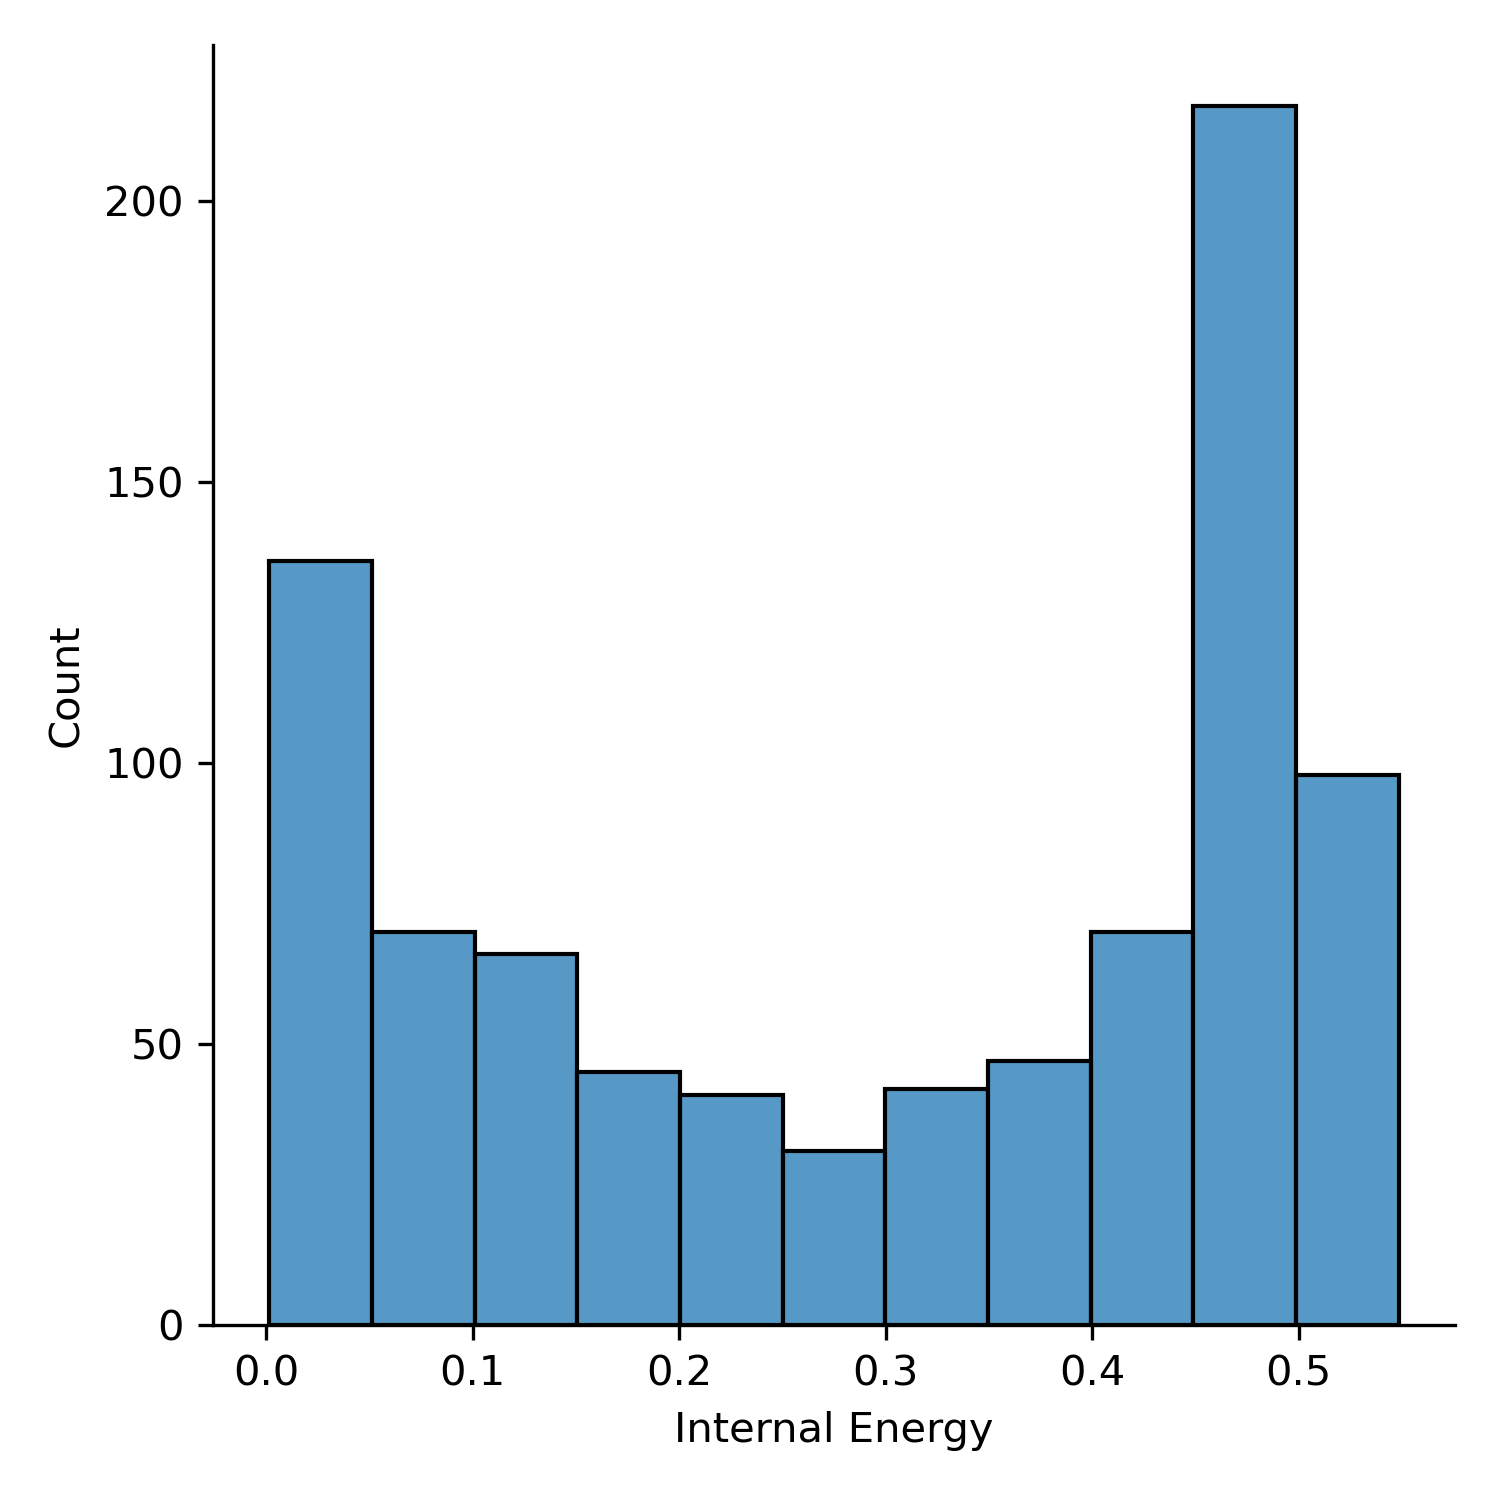
\includegraphics[width=\textwidth]{ie_cppn.png}
		\caption{Internal energy distribution of CPPNs}
	\end{subfigure}
	\caption[Constraint and internal energy distribution comparison]{Constraint and internal energy distribution comparison between random, L-System and CPPN unit generation}
	\label{fig:ciecomp}
\end{figure}

The system energy distribution is consistent across all unit generation methods. The L-System and CPPN unit generation methods are capable of adequately exploring the design space.



\section{Scale Invariance}

Scale invariance in the context of this project refers to the capability of generated units to exhibit similar behaviours at differing resolutions and dimensions. Unit layouts are defined with simple, efficient and adaptable encodings.

\subsection{Single Units}

Unit resolution may be decreased or increased while maintaining the same unit generation encoding. A lower bound exists beyond which units will no longer exhibit similar behaviour to the same unit at higher resolutions.

\subsubsection{L-Systems}

L-Systems have the potential to be scale invariant with an increase in unit size and resolution. L-Systems are constructed on the principle of recursiveness.

As unit resolution increases, L-System iterations may be increased. Longer words will result which will be interpreted as larger patterns. Patterns will have similar but not identical layouts. Figure~\ref{fig:lsinti} illustrates a simple L-System described in Table~\ref{tab:exlspar} interpreted at increasing iteration numbers.

% Please add the following required packages to your document preamble:
% \usepackage{booktabs}
% \usepackage{multirow}
\begin{table}[H]
\centering
\caption{Example L-System parameters}
\label{tab:exlspar}
\begin{tabular}{@{}lcl@{}}
\toprule
\multicolumn{1}{c}{\textbf{Parameter}} & \multicolumn{2}{c}{\textbf{Value}}                        \\ \midrule
Axiom                                  & \multicolumn{2}{c}{{[}F{]}++++{[}F{]}}                    \\ \cmidrule(l){2-3} 
\multirow{3}{*}{Grammar}               & \textbf{Variable}     & \multicolumn{1}{c}{\textbf{Rule}} \\ \cmidrule(l){2-3} 
                                       & \multicolumn{1}{l}{F} & FF++f                             \\
                                       & \multicolumn{1}{l}{f} & --FFF                             \\ \bottomrule
\end{tabular}
\end{table}

\begin{figure}[ht]
	\centering
	\begin{subfigure}[t]{0.3\textwidth}
		\centering
		
\includegraphics[width=\textwidth]{si_ls_2.png}
		\caption{2 iterations}
	\end{subfigure}
	\hfill
	\begin{subfigure}[t]{0.3\textwidth}
		\centering
		
\includegraphics[width=\textwidth]{si_ls_3.png}
		\caption{3 iterations}
	\end{subfigure}
	\hfill
	\begin{subfigure}[t]{0.3\textwidth}
		\centering
		
\includegraphics[width=\textwidth]{si_ls_4.png}
		\caption{4 iterations}
	\end{subfigure}
	\hfill
	\begin{subfigure}[t]{0.3\textwidth}
		\centering
		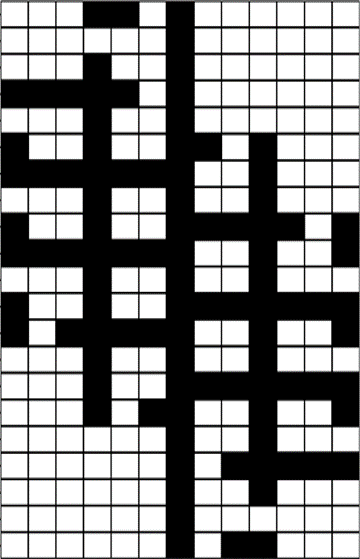
\includegraphics[width=\textwidth]{si_ls_5.png}
		\caption{5 iterations}
	\end{subfigure}
	\hfill
	\begin{subfigure}[t]{0.3\textwidth}
		\centering
		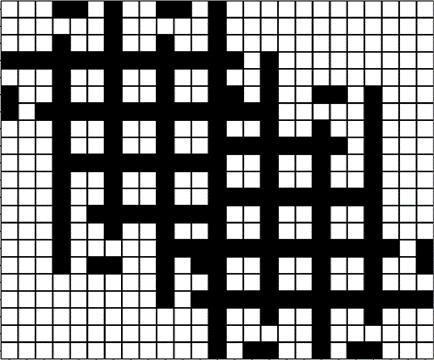
\includegraphics[width=\textwidth]{si_ls_6.png}
		\caption{6 iterations}
	\end{subfigure}
	\hfill
	\begin{subfigure}[t]{0.3\textwidth}
		\centering
		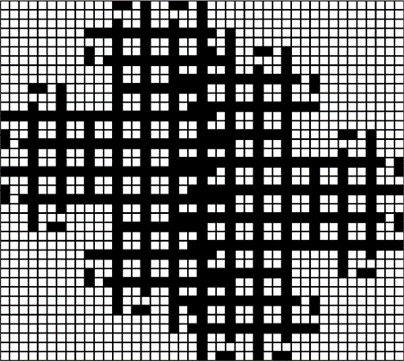
\includegraphics[width=\textwidth]{si_ls_8.png}
		\caption{8 iterations}
	\end{subfigure}
	\caption[Example L-System interpretation for different iteration values]{Example L-System from Table~\ref{tab:exlspar} interpretation for different iteration values. L-System interpretation is centred around $\left (0,0  \right )$ and is unbounded. Included elements are solid black squares and removed elements are empty white squares}
	\label{fig:lsinti}
\end{figure}

The example L-System shape only becomes consistent from 5 iterations onwards. At lower iterations, it is not clear what the L-System behaviour may be. L-Systems must be inspected on a case-by-case basis to determine from which number of iterations they become scale-invariant.

\subsubsection{CPPNs}

CPPNs are inherently scale invariant. The CPPN resolution is defined as an initial parameter. Increasing the resolution refines the model produced by the CPPN.

\subsection{Unit Grids}

Units are modelled in a $5\times 5$ unit arrangement. Unit behaviour is analyzed in this context. Results regarding system energies are obtained from these simulations. Unit deformation is impacted by the surrounding identical units. Unit deformation may be assumed to be consistent with sufficient numbers of surrounding units. Internal units display consistent behaviour, with only external units displaying major ballooning effects. Figure~ illustrates an example unit configuration with internal pressure applied.